% algorithmen/algo.tex
% Genutzte Algorithmen (Grundalgorithmen, Besonderheiten, Probleme)
%
% Ausarbeitung zur Diplomarbeit Nr. 2035 - "Erzeugung und Evaluierung 
% von Oktalbaumstrukturen als Schnittstelle zu CAD-Programmen"
%
% Autor: Stefan Mahler 2002/2003
%   Universitaet Stuttgart, SgS
% Betreuer: Ralf Mundani

\chapter{Algorithmen}
\label{algo}
Basierend auf den Erl"auterungen zu Oktalb"aumen und zu Oberfl"achenmodellen, 
insbesondere zu B-Splines, werden die in dieser Arbeit verwendeten Algorithmen 
zur Oktalbaumgenerierung aus Oberfl"achenmodellen mit glatten und gekr"ummten 
Fl"achen n"aher beschrieben. 
Hierzu m"ussen als erstes grundlegende geometrische Algorithmen, wie die 
Lagebestimmung oder Schnitt von Objekten im Raum, erkl"art werden (Abschnitt 
\ref{algo_gl_geom}). 
Ausgehend von Punkten und Linien wird anschlie"send dargestellt, wie Drei- 
oder Vierecke (und somit Objekte mit glatter Oberfl"ache) in den Oktalbaum 
eingef"ugt werden k"onnen (Abschnitt \ref{algo_plane}). Abschlie"send widmet 
sich Abschnitt \ref{algo_spline} der Generierung von Oktalb"aumen f"ur 
K"orper mit gekr"ummter Oberfl"ache.

\section{Grundlegende geometrische Algorithmen}
\label{algo_gl_geom}
Bei vielen 'klassischen' Algorithmen werden --~wie \cite[S.399]{algo_cpp} 
vermerkt~-- "Text und Zahlen verwendet, die in den meisten Programmiersystemen 
auf nat"urliche Art dargestellt und verarbeitet werden. Tats"achlich sind 
die ben"otigten elementaren Operationen in den meisten Computersystemen 
hardwarem"a"sig implementiert. Wir werden sehen, da"s die Situation bei 
geometrischen Problemen anders ist: Selbst die einfachsten Operationen mit 
Punkten und Linien k"onnen mittels Computer schwer realisierbar sein.\\
Geometrische Probleme lassen sich leicht veranschaulichen, doch das kann 
st"orend sein. Viele Probleme, die jemand l"osen kann, der ein St"uck Papier 
betrachtet (Beispiel: Befindet sich ein gegebener Punkt innerhalb eines 
Polygons?), erfordern nichttriviale Programme. F"ur komplizierte Probleme kann 
sich (wie bei vielen anderen Anwendungen) das f"ur eine Implementation 
geeignete L"osungsverfahren durchaus stark von der f"ur einen Menschen 
geeigneten L"osungsmethode unterscheiden." 

Es existieren viele Spezialf"alle (z.B. Dreieck zu Strecke oder Punkt 
entartet), die einer gesonderten Behandlung bed"urfen. 
Andererseits finden sich f"ur geometrische Probleme viele Algorithmen 
in der Literatur, insbesondere im Internet. 
Das Beachten (bzw. Nichtbeachten) von Spezialf"allen sowie die Effizienz der 
vorgeschlagenen L"osungen ist aber meist nicht sofort ersichtlich und kann 
von Anwendunsszenario zu Anwendungsszenario variieren. Die Missachtung 
von Spezialf"allen ist ein h"aufiger Programmierfehler. 

Dennoch lassen sich einige Prinzipien f"ur alle geometrischen Algorithmen 
formulieren: Fast immer wird auf Mittel der Vektorrechnung zur"uckgegriffen. 
Damit wird auch meist das Problem sehr anschaulich beschrieben. Die L"osung 
ist auch einfach auf h"oherdimensionale analoge Probleme anwendbar. 
(Allerdings gibt es manchmal L"osungen, die sich anderer geometrischer 
Beziehungen bedienen, die effizienter sind und direkt (ohne Sonderbehandlung) 
mehr Spezialf"alle abdecken). Algorithmen mit Ganzzahlarithmetik sind aus 
Effizenzgr"unden ihren Flie"skommapendants vorzuziehen. Laufvariablen 
sollten zur Vermeidung von Akkumulationsfehlern nie Flie"skommazahlen sein. 
Besonderes Augenmerk verdient die diskrete Aufteilung des Raums in Zellen. 
Allgemein sind Rundungsfehler und weitere numerische Probleme 
(z.B. Ausl"oschung) zu beachten. 
Wichtig ist hier die Frage nach der notwendigen Genauigkeit der L"osung. 
Die Analyse unterschiedlicher Algorithmen zu einem geometrischen Problem 
kann deshalb wichtig sein.

Nachfolgend sollen einige verwendete geometrische Algorithmen vorgestellt 
werden.

%%%%%%%%%%%%%%%%%%%%%%%%%%%%%%%%%%%%%%%%%%

% algorithmen/lagebest.tex
% Lagebstimmung geometrischer Objekte im Raum
%
% Ausarbeitung zur Diplomarbeit Nr. 2035 - "Erzeugung und Evaluierung 
% von Oktalbaumstrukturen als Schnittstelle zu CAD-Programmen"
%
% Autor: Stefan Mahler 2002/2003
%   Universitaet Stuttgart, SgS
% Betreuer: Ralf Mundani

\subsection{Lagebestimmung geometrischer Objekte}
\label{lagebest}
Die Bestimmung der Lage eines Objekts bez"uglich eines anderen hat zur 
Oktalbaumgenerierung eine herausragende Bedeutung. Schlie"slich wird 
die Geometrie des Oktalbaums "uber die Frage '\emph{Befindet sich das Objekt 
ganz innerhalb oder au"serhalb oder teilweise inner-/au"serhalb einer 
bestimmten Zelle?}' definiert. 

\subsubsection{Punkt-in-Zellen-Test}
Um einen Punkt einer Zelle zuordnen zu k"onnen, m"ussen die realen Koordinaten 
des Punkts im gegebenen CAD-Modell auf die Koordinaten des virtuellen Gitters 
abgebildet werden. Die Abbildung der CAD-Punkte auf das Gitter soll als 
\type{GeomPoint} bezeichnet werden. 

\begin{description}
\item[Zuordnung eines realen Punktes zu einer Zelle unterster Baumebene]~\\
\label{point_in_cell_lowest_level}
Zun"achst wird von Zellen der tiefsten Ebene ausgegangen. Sie besitzen die 
Knotenh"ohe $h_{\mbox{idx}}=0$ bzw. die Tiefe $d_{t_{\max}}$. 
In jeder Achsrichtung befinden sich $2^{d_{t_{\max}}}$ Zellen, die mit $0$ 
beginnend durchnummeriert seien. 
F"ur einen beliebigen Zellindex $\mbox{\bf idx}$ dieser Ebene gilt deshalb 
\gl{gl_idx_in_octree_basenode}{\mbox{\bf idx} \in \left[ \left( 
	\left(0\right)^{\dim} | ~ 0 \right) ; \left( 
	\left(2^{d_{t_{\max}}} - 1\right)^{\dim} | ~ 0 \right) 
    \right]\mbox{.}} 
Nachbarzellen besitzen in jede Achsrichtung den Index-Abstand $1$. F"ur ein 
\type{GeomPoint} ${\bf g}$ gilt: 
\gl{gl_geompoint_idx_basenode}{{ \bf g} \in \mbox{\bf idx} : 
    { \bf g}[i] \in \left[\mbox{\bf idx}[i]; 
	\mbox{\bf idx}[i] + 1 \right) ~ 
    \land ~ h_{ \bf g} = h_{\mbox{\bf idx}} = 0%\mbox{,}~ 
%    ~\forall i \in [0; \dim)\mbox{.}
}
mit $i = 0,\dots, {\dim}-1$. Dabei sind ${\bf g}[i]$ und $\mbox{\bf idx}[i]$ 
die $i$-te Koordinate des \type{GeomPoint} bzw. der Anteil in $i$-Richtung des 
Index. Alle Zellen besitzen die gleiche Breite. Unter Verwendung 
\glref{gl_knotentiefe_zellgroesse} ergibt sich eine Maschenweite $\lambda$  
von \[\lambda = \max_{i \in \left[0; {\dim}\right)} { \left\{ 
    { \bf p}_{\max}[i] - { \bf p}_{\min}[i] \right\} } ~ / 
    ~ 2^{d_{t_{\max}}}\mbox{.}\] 
Dabei enthalten ${\bf p}_{\max}$ und ${\bf p}_{\min}$ die jeweils gr"o"sten 
bzw. kleinsten Koordinaten der boundary cube. Somit kann jeder Punkt 
${\bf p}$ des CAD-Modells mit ${\bf p} \in \left[{\bf p}_{\min}; 
{\bf p}_{\max}\right)$ mit Hilfe der linearen Abbildung 
\gl{gl_p_to_g_using_lambda}{{\bf g} = ({ \bf p} - { \bf p}_{\min}) 
    ~ / ~ \lambda}
als entsprechender \type{GeomPoint} ${\bf g}$ dargestellt werden. 
Wird ${\bf p}_{\min}$ durch 
\gl{gl_p_min}{{ \bf p}_{\min} = \left( \min_{{ \bf p}} 
    \left\{ { \bf p}[i] \right\} \right)^{i = 0,\dots,\dim - 1}}
bzw. ${\bf p}_{\max}$ durch 
\gl{gl_p_max}{{ \bf p}_{\max} = \left( \max_{{ \bf p}} 
    \left\{ { \bf p}[i] \right\} \right)^{i = 0,\dots,\dim - 1}} 
definert, k"onnen jedoch die Punkte nicht in den Oktalbaum abgebildet werden, 
die mindestens eine ${\max}$-Koordinate enthalten. Das sind alle Punkte der 
drei Randfl"achen der boundary cube $x = { \bf p}_{\max}[0]$, $y = 
{ \bf p}_{\max}[1]$ bzw. $z = { \bf p}_{\max}[2]$. Solche Punkte w"urden einer 
Zelle zugeordnet, die wegen \glref{gl_geompoint_idx} einen Index-Anteil 
von $2^{d_{t_{\max}}}$ ergeben und mit \glref{gl_idx_in_octree} au"serhalb 
des Oktalbaums liegen. Eine L"osung w"are, ${\bf p}_{\max}$ in jeweils jede 
Achsrichtung um $\epsilon : \epsilon > 0$ nach 'rechts' zu verschieben, also 
${\bf p}_{\max}$ anstatt mit Hilfe von \glref{gl_p_max} durch 
\[{ \bf p}_{\max} = \left( \max_{{ \bf p}} 
    \left\{ { \bf p}[i] \right\} + \epsilon \right)^{i = 0,\dots,\dim - 1}\] 
zu definieren. Der "ubersch"ussige relative Anteil w"are dann jedoch vom 
CAD-Modell abh"angig. Besitzt die Geometrie nur kleine Abmessung, w"are dieser 
Anteil unn"otig gro"s. Alternativ wird die Maschenweite auf 
\gl{gl_lambda_basenode}{\lambda = { \max_{i \in \left[0; {\dim}\right)} 
    { \left\{ {\bf p}_{\max}[i] - { \bf p}_{\min}[i] \right\} } ~ 
    \over ~{ 2^{d_{t_{\max}}} - \epsilon } } }
vergr"o"sert. Um eine besonders kleine Maschenweite zu erhalten, wird 
$\epsilon \ll 1$ gesetzt. 

Der \type{GemPoint} ${\bf g}$ befindet 
(vgl. \glref{gl_geompoint_idx_basenode}) sich in der Zelle mit dem 
Index $\mbox{\bf idx}$ 
\gl{gl_gp_to_idx}{\mbox{\bf idx} = \trunc{{ \bf g}}\mbox{.}}

\item[Verallgemeinerung auf beliebige Zellebenen]\label{point_in_cell_allg}~\\
Die im letzten Punkt gemachten Betrachtungen lassen sich auf beliebige 
Zell\-ebenen "ubertragen. Es gelten dementsprechend f"ur beliebige H"ohen des 
die Zelle repr"asentierenden Oktalbaumknotens $h$ (bzw. Tiefen $d$) analog zu 
\glref{gl_idx_in_octree_basenode}, \glref{gl_geompoint_idx_basenode} und 
\glref{gl_lambda_basenode}:
\gl{gl_idx_in_octree}{\mbox{\bf idx} \in \left[ \left( \left(0\right)^{\dim} 
	| ~ h \right) ; \left( \left(2^d - 1\right)^{\dim} | ~ h \right) 
    \right]\mbox{,}} 
\gl{gl_geompoint_idx}{{\bf g} \in \mbox{\bf idx} : 
    { \bf g}[i] \in \left[\mbox{\bf idx}[i]; 
	\mbox{\bf idx}[i] + 1 \right) ~ 
    \land ~ h_{ \bf g} = h_{\mbox{\bf idx}}}
mit $i = 0, \dots ,\dim-1$ bzw.
\gl{gl_lambda}{\lambda = { \max_{i \in \left[0; {\dim}\right)} 
    { \left\{ {\bf p}_{\max}[i] - { \bf p}_{\min}[i] \right\} } ~ 
    \over ~{ 2^d - \epsilon } } }
und somit
\gl{gl_p_to_g_allg}{{\bf g} = \left( ({ \bf p} - { \bf p}_{\min}) 
    ~ * ~ \frac{2^d - \epsilon }{ \max_{i \in [0,\dots,\dim-1)} \left\{ 
	{ \bf p}_{\max}[i] - { \bf p}_{\min}[i] \right\} } 
    \left|\right. h \right)\mbox{.}}

\item[Zuordnung des Zellindex zu einem \type{GeomPoint}]~\\
$g_{\mbox{\bf idx}_{\downarrow}} = \mbox{\bf idx}$ liefert den 'rechten 
unteren vorderen' \type{GeomPoint} der Zelle $\mbox{\bf idx}$.  
Als \type{GeomPoint} $g_{\mbox{\bf idx}}$ einer Zelle wird h"aufig ihr 
Mittelpunkt definiert. Wir setzen 
\gl{gl_idx_to_geompoint}{g_{\mbox{ \bf idx}} = \mbox{ \bf idx} 
    + \left( \onehalf \right)^{\dim}\mbox{.}}

\item[Punktgleichheit]~\\
Wann sind zwei Punkte ${\bf g}_1$ und ${\bf g}_2$ im Oktalbaum als identisch 
anzusehen? Zum einem k"onnte man zwei Punkte als gleich betrachten, wenn sie 
zur gleichen Zelle geh"oren, also $\trunc{{\bf g}_1} = \trunc{{\bf g}_2}$. 
Unter anderem f"ur den \vpageref{point_in_plane_test} behandelten 
\emph{Punkt-in-Ebene-Test} eignet sich eine Abstandsbeziehung besser. 
Die Eckpunkte einer Zelle ${\bf g}_{{\mbox{ \bf idx}^{\ast}}}$ haben vom 
Mittelpunkt ${\bf g}_{\mbox{\bf idx}}$ einen Abstand $a = \sqrt{3 * 
{\onehalf}^2}$. Wir definieren 
\gl{gl_geompoint_equ}{ { { \bf g}_1 = { \bf g}_2 } ~ \equival ~
    { \left| { \bf g}_1 - { \bf g}_2 \right|^2 < \threequarters }\mbox{.}}
\end{description}

\subsubsection{Punkt-auf-Strecke-Test}
Ein Punkt ${\bf Q}$ befindet sich auf der Strecke $\overline{{\bf A}{\bf B}}$
falls
\begin{itemize}
\item ${\bf Q}$ ein Endpunkt der Strecke ist, also ${\bf Q} = {\bf A}$ oder 
    ${\bf Q} = {\bf B}$, oder 
\item ${\bf Q}$ sich auf der Geraden, die durch ${\bf A}$ und 
    ${\bf B}$ verl"auft, befindet und zwischen ${\bf A}$ und ${\bf B}$ liegt.
\end{itemize}

${\bf Q}$ liegt auf der Geraden ${\bf A}{\bf B}$, wenn der Fu"spunkt 
${\bf F}_{\bf Q}$ zu ${\bf Q}$ auf der Geraden ${\bf A}{\bf B}$ mit ${\bf Q}$ 
zusammenf"allt, also gilt
\gl{gl_q_at_line}{{ \bf Q} = { \bf F}_{ \bf Q}\mbox{.}}
Der Fu"spunkt kann mit Hilfe des Skalarprodukts berechnet werden:
\gl{gl_footpoint_at_line}{ \vct{O{F_Q}} = \frac{ < \vct{AQ}; \vct{AB} > }{%
	| \vct{AB} |^2 } ~ \vct{AB} \: + \: \vct{OA}\mbox{.}}

Ein Punkt ${\bf Q}$, der sich auf der Geraden ${\bf A}{\bf B}$ befindet, liegt 
zwischen ${\bf A}$ und ${\bf B}$, wenn gilt: 
\gl{gl_footpoint_at_stretch}{ | \overline{AQ} | < | \overline{AB} | ~ 
    \land ~ | \overline{QB} | < | \overline{AB} |\mbox{.}}

\subsubsection{Punkt-in-Ebene-Test}
\label{point_in_plane_test}
Im Folgenden werden zwei Methoden erl"autert, um zu bestimmen, ob sich ein 
Punkt ${\bf Q}$ in der Ebene $E$, die durch die Punkte ${\bf A}$, 
${\bf B}$ und ${\bf C}$ gegeben ist, befindet.
Dabei ist zu beachten
\begin{enumerate}
\item\textbf{Sonderf�lle:} Sind ${\bf A}$, ${\bf B}$ und ${\bf C}$ kollinear 
    (oder gar identisch), so ist undefiniert, ob ${\bf Q}$ in $E$ liegt. 
\item\textbf{\emph{'Abstandsregel'}:} Der Punkt-in-Ebene-Test wird 
    insbesondere dazu benutzt, um zu bestimmen, ob $E$ durch eine Zelle mit 
    dem Index ${\bf i}$ verl"auft. Der Zelle wird der Punkt ${\bf g}_i$ 
    zugeordnet, der den Mittelpunkt der Zelle darstellt. Verl"auft die Ebene 
    nicht durch den Zellmittelpunkt sondern lediglich durch die 
    Zellrandfl"ache, muss dennoch die Zelle als zur Ebene geh"orig angesehen 
    werden. Deshalb werden Punkte, die in einen Abstand 
    von $\le\onehalf$ zu $E$ besitzen, mit zur Ebene $E$ gerechnet.
\end{enumerate}

\begin{description}
%\renewcommand\item{\item ~\\}
\item["Uber den Fu"spunkt] \label{descr_in_plane_footpoint}~\\ 
    Gilt f"ur den Fu"spunkt ${\bf F}_{\bf Q}$ des Punktes ${\bf Q}$ auf der 
    Ebene $E$
    \gl{gl_point_in_plane_via_f}{{ \bf F}_{ \bf Q} = { \bf Q}\mbox{,}}
    dann liegt ${\bf Q}$ in $E$. 
    ${\bf F}_{\bf Q}$ kann "uber 
    \gl{gl_footpoint_in_plane}{ \vct{O{F_Q}} = \vct{OQ} ~ - ~ 
	\textstyle{ \left( \left< \vct{n_E}; \vct{OQ} \right> - d \right) } 
	\vct{n_E} }
    berechnet werden. Dabei ist $\vct{n_E}$ nach 
    \glref{gl_flaechenorientierung} der Normalenvektor der Ebene.
\item["Uber das Determinantenverfahren] \label{descr_in_plane_det}~\\ 
    Das Volumen $V$ des durch die Vektoren $\vct{a}$, $\vct{b}$ und $\vct{c}$ 
    gegebenen Spans kann durch 
    \gl{gl_vol_ueber_det}{V = \det \left(\vct{a}; \vct{b}; \vct{c}\right)}
    ermittelt werden. 
    Damit ergibt sich folgende Beziehung f"ur den Abstand $a$ des 
    Punktes ${\bf Q}$ zur Ebene $E$ 
    \gl{gl_dist_point_plane}{\det{}^2 \left(\vct{AB}; \vct{AC}; \vct{AP}\right) 
	< a^2 ~ \left| \vct{AB} \crossprod \vct{AC} \right|^2\mbox{.}} 
    Mit einem maximal zul"assigen Abstandsquadrat von $a^2 = \onehalf$ ergibt 
    sich
    \gl{gl_point_in_plane_via_det}{{ \bf Q} \in E ~ \Longleftrightarrow ~ 
	\det{}^2 \left(\vct{AB}; \vct{AC}; \vct{AP}\right) 
	\le \onehalf ~ \left| \vct{AB} \crossprod \vct{AC} \right|^2\mbox{.}} 
\end{description}

\subsubsection{Punkt-in-Polygon-Test}
F"ur den Test, ob sich ein Punkt ${\bf Q}$ in einem \emph{beliebigen} Polygon 
befindet, bietet sich die \textbf{Strahlmethode} an:

Sei ein Polygon $H$ durch den geschlossenen Streckenzug 
$\overline{{\bf p}_0{\bf p}_1}$ $\dots$ 
$\overline{{\bf p}_{n-2}{\bf p}_{n-1}}$ $\overline{{\bf p}_{n-1}{\bf p}_n}$ 
mit ${\bf p}_n = {\bf p}_0$ gegeben. Dann kann mit Hilfe des Teststrahls 
$\strch{{\bf Q}{\bf W}}$ "uberpr"uft werden, ob ${\bf Q}$ auf dem Rand, 
innerhalb oder au"serhalb von $H$ liegt. Dabei muss garantiert sein, dass 
sich ${\bf W}$ au"serhalb von $H$ befindet. Zu diesem Zweck wird ${\bf W}$ 
am besten auf eine Position au"serhalb der boundary cube festgelegt, z.B. : 
${\bf W} = \left({\bf Q}[0]; {\bf Q}[1]; 2^{d_{\bf Q}} | h_{\bf Q}\right)$.
Nun wird f"ur alle Streckenz"uge $\overline{{\bf p}_{i}{\bf p}_{i+1}}$ mit 
$i= 0,\dots,n-1$ "uberpr"uft, ob sie den Teststrahl schneiden. 
Liegt ${\bf Q}$ auf einem Streckenzug, liegt ${\bf Q}$ auf dem Polygonrand 
und der Test kann abgebrochen werden. Ist ansonsten die Anzahl der Schnitte 
gerade, dann liegt ${\bf Q}$ innerhalb, ist die Anzahl der Schnitte ungerade, 
befindet sich ${\bf Q}$ au"serhalb des Polygons, also gilt: 
\gl{gl_point_in_polygon_via_ray}{{ \bf Q} \cases{
    \mbox{on} ~ H\mbox{,} & { \bf Q} \in \overline{{ \bf p}_i{ \bf p}_{i+1}}\\
    \mbox{in} ~ H\mbox{,} & \nu \mod 2 = 0\\
    \notin    ~ H\mbox{,} & \nu \mod 2 = 1}\mbox{.}}
Dabei ist $i= 0,\dots,n-1$ und $\nu$ die Anzahl der Schnitte. Folgende 
Sonderf"alle sind zu beachten: Ein Streckenzug wird in einem Eckpunkt vom 
Teststrahl geschnitten oder f"allt mit dem Teststrahl zusammen. Diese F"alle 
werden genau dann als Schnitt gez"ahlt, wenn es im Folgenden zu einem 
Seitenwechsel bez"uglich des Teststrahls kommt.

\label{polyeder_test}
Das Verfahren l"asst sich auch auf beliebige \textbf{Polyeder} (dann mit Test 
auf Schnitt der Teil\-oberfl"achen) "ubertragen. 

Alternativ l"asst sich das Verfahren leicht abwandeln, wenn man die 
\emph{Orientierung} der Polygon-/Polyeder-R"ander ausnutzt 
(\textbf{Teststrahlmethode}). Jetzt muss nur der zu ${\bf Q}$ am n"achsten 
gelegene Streckenzug bzw. die zu ${\bf Q}$ am n"achstengelegene 
Teiloberfl"ache\footnote{wieder entlang eines Teststrahls oder alternativ 
der/die allgemein am n"achsten gelegene Streckenzug bzw. Teil\-oberfl"ache} 
ermittelt werden. Dann kann mit Hilfe des unten 
beschriebenen Tests der \emph{Lage eines Punktes bez"uglich einer Ebene} 
(als Basispunkt der Ebene den Schnittpunkt ${\bf S}$ einsetzen) bestimmt 
werden, ob sich der Punkt innerhalb oder au"serhalb des Polyeders befindet. 
Liegt ${\bf Q}$ in der Ebene der Teiloberfl"ache, so wird diese Fl"ache 
einfach unber"ucksichtigt gelassen. Der Sonderfall ${\bf Q}$ liegt in der 
Teilfl"ache wurde zuvor durch ${\bf Q} = {\bf S}$ "uberpr"uft. Befindet 
sich ${\bf Q}$ in der Ebene, aber nicht auf der Teilfl"ache, muss es 
mindestens eine weitere Fl"ache geben, die genauso weit von ${\bf Q}$ entfernt 
ist, deren Ebene jedoch nicht mit dem Teststrahl $\strch{{\bf Q}{\bf S}}$ 
zusammenf"allt. Kann keine n"achstliegende Fl"ache gefunden werden, befindet 
sich ${\bf Q}$ au"serhalb des Polyeders. 
Prinzipiell l"asst sich das Verfahren auch auf Objekte mit gekr"ummten Rand 
"ubertragen. Dabei ist jedoch -- neben der schwereren Schnittpunktermittlung 
-- zu beachten, dass mehrere Schnittpunkte (nicht nur im Sonderfall des 
Zusammenfallens von Streckenzug/Fl"achenst"uck mit dem Teststrahl) 
existieren k"onnen. Des Weiteren ist die Orientierung gekr"ummter Fl"achen 
i.A. nicht global gleich und muss dehalb am entsprechenden Schnittpunkt 
ermittelt werden. 

Werden nicht beliebige, sondern nur \emph{konvexe Polygone} eingesetzt, 
k"onnen effizientere oder einfachere Verfahren gefunden werden: 

Besonders effizient ist dabei das \textbf{Umlaufsinnverfahren}. 
Sei ein Dreieck $H= \triangle{\bf A}{\bf B}{\bf C}$ im 
\emph{Zweidimensionalen} gegeben. 
Der Punkt ${\bf Q}$ befindet sich genau dann in $H$, wenn der Umlaufsinn der 
Dreiecke die durch Ersetzen von jeweils einem der Punkte ${\bf A}$, ${\bf B}$ 
bzw. ${\bf C}$ durch ${\bf Q}$ entstehen, mit dem Umlaufsinn von $H$ identisch 
ist, also 
\gl{gl_point_in_triangle_ccw}{\func{ccw}{{\large H}} = 
    \func{ccw}{$\triangle${\bf Q}{\bf B}{\bf C}} = 
    \func{ccw}{$\triangle${\bf A}{\bf Q}{\bf C}} = 
    \func{ccw}{$\triangle${\bf A}{\bf B}{\bf Q}}\mbox{.}}
Dabei ist \func{ccw}{} ein Funktion, die zu einem Dreieck seinen 
Umlaufsinn bestimmt. Die Umlaufsinnbestimmung kann im zweidimensionalen 
Fall mit Hilfe des Skalarprodukts sehr effizient geschehen (vgl. 
\cite{algo_cpp}). Die "Ubertragung ins Dreidimensionale erweist sich als 
schwieriger. Hier gibt es keine nat"urliche Definition des Uhrzeigersinns. 
Als L"osung k"onnten im Falle, dass ${\bf Q}$ in der Ebene des Dreiecks $H$ 
liegt, die betreffenden Punkte in einer (zweidimensionalen) Basis 
zweier Ebenenvektoren dargestellt werden. Alternativ k"onnten die Richtungen 
der Normalvektoren der Dreiecke verglichen werden.

\label{point_in_polygon_angle}
\cite{point_in_polygon} stellt das in dieser Arbeit verwendete 
\textbf{Winkelverfahren} vor. Ein Punkt ${\bf Q}$, der in der Ebene $E$ des 
konvexen Polygons $H$ liegt, befindet sich genau dann innerhalb von $H$, 
wenn gilt:
\gl{gl_point_in_polygon_angle}{{\sum_{i=0}^{n-1} \arccos{
    \left<{\vct{Q{p_i}} \over |\vct{Q{p_i}}|}; 
	  {\vct{Q{p_{i+1}}} \over |\vct{Q{p_{i+1}}}|} \right>}} = 2\pi\mbox{.}}
Dabei ist wieder $\overline{{\bf p}_0{\bf p}_1}, \dots, 
\overline{{\bf p}_{n-1}{\bf p}_n}$ (mit ${\bf p}_n={\bf p}_0$ und 
${\bf Q} \notin \overline{{{\bf p}_i}{{\bf p}_{i+1}}}$) der den Rand 
von $H$ definierende geschlossen Streckenzug. 

F"ur konvexe Polygone kann auch das \textbf{Eckpunkt-Schnittverfahren} 
verwendet werden. 
Ein Punkt ${\bf Q}$ der sich nicht auf dem Polygonrand befindet, liegt genau 
dann im Polygon $H$, welches durch den Streckenzug 
$\overline{{\bf p}_0{\bf p}_1}$,\dots,$\overline{{\bf p}_{n-1}{\bf p}_n}$ 
mit ${\bf p}_n={\bf p}_0$ gegeben ist, wenn gilt
\gl{gl_point_in_polygon_corner_intersect}{%
    \forall i \in [0; n) \forall k \in [0; n) \setminus \{i; i+1\}:
    \overline{{\bf Q}{\bf p}_i} \land \overline{{\bf p}_k{ \bf p}_{k+1}}
    = \emptyset\mbox{,}} 
also keine Strecke $\overline{{\bf Q}{\bf p}_i}$ durch einen Streckenzug des 
Polygons $\overline{{\bf p}_k{\bf p}_{k+1}}$ geschnitten wird.

\subsubsection{Lage eines Punktes bez"uglich einer Fl"ache}
Aus der Orientierung der Fl"achen nach \glref{gl_flaechenorientierung} ergibt 
sich f"ur alle Fl"achen eine Innen- und Au"senseite. 
F"ur einen Punkt ${\bf Q}$, der sich nicht auf der Ebene befindet, kann nun 
durch 
\gl{gl_point_plane_side}{{\bf Q} ~ \mathrm{is} ~ 
        \cases{\mbox{inside},  & \varphi > 0\\
	       \mbox{outside}, & \varphi < 0}}
sein Lage berechnet werden. $\varphi$ ist ein dem Winkel 
zwischen dem Normalenvektor $\vct{n_E}$ und dem Vektor zwischen ${\bf Q}$ 
und einem Fl"achenpunkt ${\bf F}$ entsprechender Wert. Es gilt 
\gl{gl_phi_from_skalar_prod}{\varphi = \left<\vct{n_E}; \vct{QF}
	\right>\mbox{.}}

%% End of Document


% algorithmen/schnitt.tex
% Schnitt zweier Linien, Schnitt Linie mit Polygon
%
% Ausarbeitung zur Diplomarbeit Nr. 2035 - "Erzeugung und Evaluierung 
% von Oktalbaumstrukturen als Schnittstelle zu CAD-Programmen"
%
% Autor: Stefan Mahler 2002/2003
%   Universitaet Stuttgart, SgS
% Betreuer: Ralf Mundani

\subsection{Schnitt geometrischer Objekte}
Im Folgenden werden einige Schnittverfahren f"ur einfache Objekte vorgestellt. 
Wie im oberen Abschnitt zu sehen ist, wird die Schnittbestimmung insbesondere 
f"ur einige Verfahren zur Lagebestimmung verwendet.

\subsubsection{Schnitt zweier Strecken}
\cite{algo_cpp} beschreibt einen besonders effizienten Algorithmus, der  
"uberpr"uft, ob sich zwei Strecken $\overline{{\bf A}{\bf B}}$ und 
$\overline{{\bf C}{\bf D}}$, die sich in einer Ebene befinden, schneiden. 
Der Einfachheit halber soll verlangt sein, dass die Punkte 
${\bf A}$, ${\bf B}$, ${\bf C}$, ${\bf D}$ paarweise verschieden 
sind und nicht kollinear liegen. 
(Der Originalalgorithmus macht diese Einschr"ankung nicht, da hier f"ur diese 
Sonderf"alle die \func{ccw}{{}${\bf p}_1$, ${\bf p}_2$, ${\bf p}_3$} speziell 
definierte Werte liefert.)
\gl{gl_intersect_two_str_ccw}{ 
    \begin{array}{c} 
    \overline{{\bf A}{\bf B}} \; \mathrm{intersect} \; 
	\overline{{\bf C}{\bf D}} \; \equival \\
    \left( \func{ccw}{{\bf A},{\bf B},{\bf C}} = 
	\func{ccw}{{\bf B},{\bf A},{\bf D}} \right) 
     ~ \land ~ \left( \func{ccw}{{\bf C},{\bf D},{\bf A}} = 
	\func{ccw}{{\bf D},{\bf C},{\bf B}} \right) 
    \end{array}
}

\subsubsection{Schnitt einer achsparallelen Geraden mit einem Polygon}
Es soll der Schnittpunkt zwischen einer achsparallelen Geraden mit einem 
Polygon $H$ bestimmt werden, wenn ein solcher existiert. 
Hier soll auf die Mittel der Vektorrechnung zur"uckgegriffen werden. 
Die Verwendung einer achsparallelen Gerade f"ur den Schnitt hat den Vorteil, 
dass bereits zwei Koordinaten des Schnittpunkts bekannt sind.  
Es sind die jeweiligen Koordinaten der Geraden. O.B.d.A. soll eine Gerade
parallel zur z-Achse betrachtet werden, die durch den Punkt 
${\bf Q} = (x_0; y_0; z_0 | h)$ verl"auft: 
\[g = \left\{ (x_0; y_0; z | h) : z \in \Realnumbers \right\}\mbox{.}\]
Dann muss f"ur den Schnittpunkt ${\bf S}=\left(x_0; y_0; z_{\bf S}\right)$ 
gelten:
\gl{gl_S_in_polygon}{\left(x_0; y_0; z_{\bf S}\right) \in H\mbox{.}}
Die Gerade liegt in der Polygonebene oder verl"auft parallel zu ihr, falls 
\gl{gl_z_line_parallel_polygon}{\vct{n_H}[2] = 0\mbox{.}}
Solche F"alle werden im Folgenden nicht weiter betrachtet.
F"ur den Schnittpunkt gilt nun 
\gl{gl_z_s_line_polygon}{z_{\bf S} = z_0 + { \scriptstyle{ \left<
    \vct{Q{p_0}}; \vct{n_H} \right>} \over \vct{n_H}[2]}
    \mbox{.}}
Zur Bestimmung, ob der Schnittpunkt mit der Polygonebene auch im Polygon 
selbst liegt, kann die Projektion in die $xy$-Ebene betrachtet und die 
Umlaufsinnmethode angewendet werden. 
 
F"ur die Strahlmethode (im Abschnitt \emph{Punkt-in-Polygon-Test} 
\vpageref{polyeder_test} beschrieben) muss 
nun noch $z_{\bf S} > {\bf Q}[2]$ sein.

%% End of Document


% Ausarbeitung zur Diplomarbeit Nr. 2035 - "Erzeugung und Evaluierung 
% von Oktalbaumstrukturen als Schnittstelle zu CAD-Programmen"
%   
% Autor: Stefan Mahler 2002/2003
%   Universitaet Stuttgart, SgS
% Betreuer: Ralf Mundani

\section{Erzeugung von K"orpern mit glatter Oberfl"ache}
\label{algo_plane}
%Standard hierachisch <-> 'emulierte' Normzellen
%Warum: schneller?
%Probleme: hoeherer Speicheraufwand? F�llen? Blasen?

Zur Oktalbaumgenerierung wird h"aufig ein Verfahren "ahnlich dem bei 
\cite{dipl_anw_oct} verwendet: Suksessiv wird der Oktalbaum solange 
verfeinert, bis eine durch den Oktalbaum-Knoten repr"asentierte Zelle sich 
vollst"andig innerhalb oder au"serhalb des K"orpers befinden oder die 
maximale Baumtiefe erreicht wurde. Die Bl"atter werden entsprechend gef"arbt. 

Gerade bei der Verwendung von K"orpern mit gekr"ummten Fl"achen ist aber 
die Lokalisation von Punkten und damit der zu betrachtenden Zellen 
aufw"andig. Deshalb wurde innerhalb dieser Arbeit ein alternatives Verfahren 
entwickelt und analysiert. Um den Zeitaufwand zur Oktalbaumgenerierung zu 
minimieren, sollte die Anzahl der notwendigen Lagebestimmungen von 
Zellen (bez"uglich der modellierten K"orper) minimiert werden. Stattdessen 
sollte die Struktur der modellierten K"orper durch effiziente Verfahren 
in den Oktalbaum "ubertragen werden. Die Grundidee ist dabei, zuerst die 
Oberfl"ache der K"orper in die Oktalbaumstruktur zu generieren und 
anschlie"send die K"orper zu 'f�llen'.
Die Anzahl der Lagebestimmungen $\eta$ betr"agt dann idealerweise nur noch 
\gl{gl_ideal_num_pos_check}{\eta = 1 + \kappa\mbox{,}}
wenn $\kappa$ die Anzahl zusammenh"angender vollst"andig abgetrennter 
K"orpersegmente ist. Aufbauend auf dem Verfahren zur Punktegenerierung in 
Oktalb"aumen wird dargestellt, wie glatte Oberfl"achen in einer 
Oktalbaumstruktur erzeugt werden k"onnen. Danach wird auf F"ullmethoden 
eingegangen. Abschlie"send werden die 
unterschiedlichen Algorithmen zur "Ubertragung von K"orpermodellen in 
eine Oktalbaumstruktur verglichen.

\subsection{Punkte}
Das einfachste Objekt, welches in einem Oktalbaum dargestellt werden kann, 
ist ein Punkt. Dabei ist jedoch zu beachten, dass dem Punkt im Oktalbaum ein 
Volumen zugeordnet wird (n"amlich das Volumen der Zelle, in der er sich 
befindet). Da Punkte jedoch eigentlich keine Abmessungen besitzen, sind sie 
zweckm"a"siger Weise in der untersten Baumebene (also mit der 
Knotenh"ohe $h=0$) einzuf"ugen. 
Im Abschnitt \ref{point_in_cell_lowest_level} wurde bereits 
erl"autert, wie ein Punkt des CAD-Modells in einen \type{GeomPoint} ${\bf g}$, 
also in die Koordinaten des Oktalbaums, transformiert werden kann. Der Index 
${\bf g}_{\mbox{idx}}$ von ${\bf g}$ entsprach dabei dem 
Zellindex ${\bf idx}$.

Im Folgenden wird gezeigt, wie sich hieraus der Pfad durch den Oktalbaum 
zum entsprechenden Knoten bestimmen l"asst. 
Bei der Verfeinerung einer Zelle wird diese in jede Achsrichtung halbiert. 
Liegt die Sohnzelle im jeweiligen 'oberen' Teilraum, so erh"alt die 
Pfadkomponente dieser Achsrichtung $\eta_{\mbox{ax}}$ den Wert $1$ zugewiesen 
und $0$ entsprechend f"ur den 'unteren' Teilraum. Ist ${\bf g}_m$ der 
Mittelpunkt der Zelle gilt also:
\gl{gl_pathcomp_to_axpart}{\eta_{\mbox{ax}} = 
    \cases{0, & {\bf g} < {\bf g}_m \\ 1, & {\bf g} \ge {\bf g}_m}\mbox{.}}
"Uber die Pfadkomponenten f"ur jede Achsrichtung kann die Pfadnummer $\eta$ 
definiert werden:
\gl{gl_path_at_pathcomp}{\eta = \sum_{i=0}^{\dim-1} \eta_i ~ 2^i\mbox{.}}
Die Reihenfolge der Sohnknoten soll entsprechend der Pfadnummerierung 
erfolgen. F"ur den virtuellen Pfad zur Wurzel wird die Pfadnummer $0$ 
definiert. Somit hat die Wurzel auch die 'Sohnnummer' $0$.

F"ur den Index-Teil ${\mbox{\bf idx}_{\mbox{ax}}^h}$ einer Zelle f"ur die 
H"ohe $h$ in $\mbox{ax}$-Richtung ergibt sich:
\gl{gl_idx_part_at_hight}{\mbox{\bf idx}_{\mbox{ax}}^h
     = ( ~ \mbox{\bf idx}[\mbox{ax}] / 2^h ~ ) ~ \mod ~ 2
     = \cases{0, & \mbox{Zelle im 'unteren' Teilraum} \\
    	      1, & \mbox{Zelle im 'oberen' Teilraum}}\mbox{.}}
Damit gibt $\mbox{\bf idx}_{\mbox{ax}}^h$ die Sohnnummer des Knotens wieder, 
der sich auf dem Pfad zum Knoten, der die Zelle $\mbox{\bf idx}$ 
repr"asentiert, auf der H"ohe $h$ befindet 
(vgl. \algref{alg_getpart_from_idx}). 
Der Index $\mbox{\bf idx}$ ist somit eine regul"are \emph{Positionscodierung} 
(vgl. S. \pageref{pos_code}). 
Er wird deshalb auch als Index des entsprechenden Knotens (im Sinne der 
Positionscodierung) angesehen. 

\alg{alg_getpart_from_idx}{\funcdef{getPart}{idx}{PartType}}{%
\funcdef{getPart}{NodeIndex idx}{PartType}
\funcbeg
  PartType part:= \(0\)\\
  \forloop{Axis ax}{0}{\dim-1}{1}
    part:= part \(+ ~\left( \mbox{\bf idx}[\mbox{ax}] / 2^{h - 1} 
			\right) \mod 2\)\\
  \closefor
  \ret{part}
\closefunc
}

Mit Hilfe des \algref{alg_get_node_from_idx} kann zu einem Index 
der zugeh"orige Oktalbaumknoten in 
$\mathcal{O}(d_{\mbox{\bf idx}})$ und somit insbesondere in 
$\mathcal{O}(d_{t_{\max}})$ gefunden werden. 

\alg{alg_get_node_from_idx}{\funcdef{getNode}{idx}{\_octree}}{%
\pre{\func{isIn}{idx} \(\land\) \func{getExistNode}{idx} \( = \) idx}\\
\funcdef{getNode}{NodeIndex idx}{Node}
\funcbeg
  \_octree nodeAddr:= \func{getTree}{}\\
  \forloop{Hight h}{d_{t_{\max}}}{h_{\mbox{\bf idx}}}{-1}
    nodeAddr:= \func{getChild}{nodeAddr, \func{getPart}{idx}}\\
  \closefor
  \ret{nodeAddr}
\closefunc{}
}

Durch \funcdef{isIn}{NodeIndex idx}{bool} kann ermittelt werden, ob durch 
\param{idx} ein Volumen des Oktalbaums referenziert wird. Dazu wird 
\glref{gl_idx_in_octree} verwendet. 
\gl{gl_isIn_idx}{\func{isIn}{idx} = \cases{\true, & \mbox{\bf idx} \in 
    \left[ \left( (0)^{\dim} | h_{\mbox{\bf idx}} \right);
           \left( (2^{d_{t_{\max}}-h_{\scriptstyle{\mbox{\bf idx}}}}-1)^{\dim}
		| h_{\mbox{\bf idx}} \right) \right] \\
					   \false, & \mbox{sonst}}}
Im \algref{alg_getexistnode_idx} liefert \func{getExistNode}{idx}{} 
\param{idx}, falls der entsprechende 
Knoten bereits im Zeigergeflecht des Oktalbaums als Knoten eingetragen ist und 
ansonsten den Knoten mit kleinster H"ohe auf dem Pfad zu ihm, der existiert.

\alg{alg_getexistnode_idx}{\funcdef{getExistNode}{idx}{NodeIndex}}{%
\pre{\func{isIn}{idx}}\\
\funcdef{getExistNode}{NodeIndex idx}{NodeIndex}
\funcbeg
  Hight h:= \(d_{t_{\max}}\)\\
  \_octree nodeAddr:= \func{getTree}{}\\
~\\
  \whileloop{\neg \func{isLeaf}{\func{getNode}{nodeAddr}} 
	     \land h > h_{\scriptstyle{\mbox{\bf idx}}}}
    nodeAddr:= \func{getChild}{nodeAddr, \func{getPart}{idx}}\\
    h:= h - 1\\
  \closewhile
~\\
  NodeIndex retVal:= idx\\
  \forloop{Axis ax}{0}{\dim - 1}{1}
     {\bf retVal}[ax]:= {\bf retVal}[ax] \( / 2^{h - h_{\mathrm{\bf idx}}}\)\\
  \closefor
  \(h_{\mbox{retVal}}\):= h\\
  \ret{retVal}
\closefunc
}

Beim Hinzuf"ugen von Punkten zum Oktalbaum ist zu beachten, dass i.A. der 
Pfad zum hinzuzuf"ugenden Knoten teilweise existiert, der untere Teil des 
Pfads muss aber erst im Oktalbaum erzeugt werden. \algref{alg_add_point} 
zeigt ein Verfahren, das zum Hinzuf"ugen von Punkten mit dem Index 
\param{idx} und der Farbe \param{color} in den Oktalbaum verwendet werden 
kann.

\alg[!t]{alg_add_point}{\procdef{add}{idx, color}}{%
\procdef{add}{NodeIndex idx, Color color}
\procbeg
  NodeIndex leafAtPath:= \func{getExistNode}{idx}\\
  \_octree nodeAddr:= \func{getNode}{leafAtPath}\\
  \whileloop{h_{\mbox{leafAtPath}} > 0}
    PartType part:= \func{getPart}{leafAtPath}\\
    nodeAddr:= \func{createLeafs}{nodeAddr}\\
    leafAtPath:= \func{getChild}{leafAtPath, part} \\
  \closewhile
  \proc{setColor}{\func{getNode}{nodeAddr}, color}
\closeproc
}

\label{func_createleafs}
\funcdef{createLeafs}{\_octree nodeAddr}{\_octree} wird zum Erzeugen neuer 
S"ohne zu einem Blatt im Oktalbaum verwendet. Der R"uckgabewert ist eine 
Referenz auf die neuerzeugten Sohn\-knoten. Der Vater\-knoten ist 
damit --~nat"urlich~-- jetzt innerer Knoten. Es soll zun"achst davon 
ausgegangen werden, dass die Sohn\-knoten mit der 
Farbe \const{NO\_OBJECT\_COLOR} (also als 'zu keinem K"orper geh"orend') 
initialisiert werden. F"ur den  F"ullalgorithmus im Abschnitt \ref{fill_alg} 
wird allerdings eine andere Initialisierungsfarbe verwendet.

Aus einem Index l"asst sich also in $\mathcal{O}(d_{t_{\max}})$ der 
zugeh"orige Knoten ermitteln oder in den Baum einf"ugen (und damit seine 
Farbe ermitteln oder setzen). 

\label{nas_to_octree}
\algref{alg_add_point} l"asst sich auch zum 
Erzeugen eines Oktalbaums aus einem Normzellen-Aufz"ahlungsschema verwenden. 
F"ur die maximale Baumtiefe $d_{t_{\max}}$ muss gelten: 
\gl{gl_bez_dt_max_normzellen}{\nu = 2^{d_{t_{\max}}}\mbox{,}}
wenn $\nu$ die Anzahl der als W"urfel gegebenen Normzellen in jeder 
Achsrichtung ist. F"ur die Konvertierung des gesamten 
Normzellen-Aufz"ahlungsschemas ist somit 
\mbox{\(\mathcal{O}(d_{t_{\max}}*2^{\dim*d_{t_{\max}}}) 
    = \mathcal{O}(\log(\nu)*\nu^3)\)} Zeit notwendig. 
Der gleiche Zeitaufwand ist auch f"ur die andere Richtung --~die 
Konvertierung des Normzellen-Aufz"ahlungsschemas aus einem 
Oktalbaum~-- notwendig. Hierzu m"ussen lediglich die 
Funktionen \func{getExistNode}{} (vgl. \algref{alg_octree_to_nas}) 
und \func{getColor}{} verwendet werden.

\alg[!t]{alg_octree_to_nas}{%
    \funcdef{octree2nas}{}{\field{[][][]}{Color}}}{%
\funcdef{octree2nas}{}{\field{\((0..\nu-1)^{\dim}\)}{Color}}
\funcbeg
  \field{\((0..\nu-1)^{\dim}\)}{Color} colors\\
  \forloop{AxIndex z}{0}{\nu-1}{1}
    \forloop{AxIndex y}{0}{\nu-1)}{1}
      \forlooptext{AxIndex x}{0}{\nu-1}{1}\\
      ~~NodeIndex idx:= \((x; y; z | 0)\)\\
      ~~idx:= \func{getExistNode}{idx}\\
      ~~colors[x][y][z]:= \func{getColor}{idx}\\
      \closefortext
    \closefor
  \closefor
  \ret{colors}
\closefunc
}

\subsection{Linien}
Zum Erzeugen von Linien im Oktalbaum kann auf das Generieren von Punkten 
aufgebaut werden. 

Um einer Strecke $\overline{AB}$ im Oktalbaum darzustellen, 
muss in alle Zellen, durch die die Strecke f"uhrt, ein Punkt eingef"ugt 
werden. 

{
\let\mywidth=\linewidth
\parbox[t]{0.7\linewidth}{%
Aus dem Bereich der Rastergrafik ist der Bresenham-Algorithmus 
bekannt. 
Eine Linie von einem Anfangspunkt ${\bf A}$ zu einem 
Endpunkt ${\bf B}$ wird "uber 
das Raster auf der $xy$-Ebene approximiert, 
indem sukzessive zu dem direkten 
oder diagonalen Nachbar gegangen wird, der  
in Richtung ${\bf B}$ der Ideallinie am n"achsten 
liegt. 
Die 
ausschlie"sliche Nutzung ganzer Zahlen ist eine weitere Eigenschaft des 
Bresenham-Algorithmus (vgl. Abb. \ref{abb_bresenham}). 
}
\hspace{1em}
\parbox[t][4.5cm][c]{0.25\mywidth}{%
    \begin{center}
     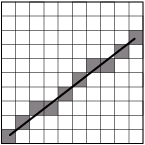
\includegraphics[width=0.85\linewidth]{scanline_bresenham} 
    \end{center}
    \begin{center}
    \renewcommand\figurename{Abb.}
    \setcapindent{1em}
    \captionof{figure}{Bresenham-Algorithmus}
    \label{abb_bresenham}
    \vspace{1em}
    \end{center}
}
}

{
\let\mywidth=\linewidth
\parbox[t]{0.7\linewidth}{%
    In der digitalen Regelungstechnik zum Verfahren von Strecken kommt ein 
    "ahnliches Verfahren zum Einsatz. 
    Hierbei wird jedoch das zu regelnde Teil nur entlang einer 
    Koordinatenachse gleichzeitig bewegt. 
    W"ahrend der Bresenham-Algorithmus $16$ Fallunterscheidungen (f"ur jede 
    Koordinatenachse, jede Winkelhalbierende und jede Fl"ache zwischen ihnen 
    f"ur beide Richtungen) macht, werden in dieser Alternative alle F"alle 
    gleichartig behandelt. 
    Des Weiteren ist die "Ubertragung ins 3-Dimensionale hier einfach. 
    Das benutzte Verfahren lehnt sich stark an das Alternativverfahren an
    (vgl. Abb. \ref{abb_scan_line}). 
}
\hspace{1em}
\parbox[t][5cm][c]{0.25\mywidth}{%
    \begin{center}
    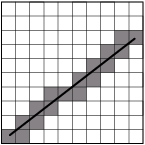
\includegraphics[width=0.85\linewidth]{scanline_alt}
    \end{center}
    \begin{center}
    \renewcommand\figurename{Abb.}
    \setcapindent{1em}
    \captionof{figure}{Scan-Line-Basisverfahren dieser Arbeit}
    \label{abb_scan_line}
    \vspace{1em}
    \end{center}
}
}

Unabh"angig vom konkret benutzten Verfahren gelten folgende Beziehungen: 
\begin{itemize} 
\item Aus dem Differenzvektor $\Delta = {\bf B} - {\bf A}$ l"asst sich 
die Steigung bzw. das Steigungsverh"altnis der Strecke ermitteln.
\item Es wird immer eine Nachbarzelle/ein Nachbarpunkt gesucht. Der Abstand 
    zwischen zwei Nachbarpunkten auf einer Koordinatenachse ist nie 
    gr"o"ser als $1$. Daraus ergibt sich der zusammenh"angende Verlauf 
    der entstehenden Kurve.
\item Da $\Delta$ die Richtung von $\strch{AB}$ festlegt, ist somit auch 
    die Richtung gegeben, in welcher auf der jeweiligen Koordinatenachse 
    der Nachbar gesucht werden muss.
\item Im Allgemeinen wird die $\strch{AB}$ durch eine treppenartige Kurve 
    angen"ahert, die von ${\bf A}$ ausgeht und in ${\bf B}$ endet. 
    F"ur jeden Punkt der Kurve ergibt sich zur 
    Ideallinie: $\strch{AB}~ \equiv \{{\bf p} : 
    {\bf p} = {\bf A} + \tau~ \Delta \}$ mit $\tau \in [0, 1]$. 
    Damit kann ein Fehler $\eta$ zu jedem Kurvenpunkt ermittelt werden.
    Es gilt:
    \gl{gl_error_in_beg_and_end_point}{\eta_{\bf A} = \eta_{\bf B} = 0}
    und f"ur einen beliebigen Punkt
    \gl{gl_error_bel_punkt}{\eta \ge 0\mbox{.}} 
    Als jeweils n"achsten Punkt wird immer der mit $\eta=\eta_{\min}$ (also 
    minimalen Fehler) aus einer Menge ausgesucht. (Falls es mehrere solche 
    Punkte gibt, wird der erstbeste von ihnen genommen.)
\end{itemize}

\label{descr_scan_line}
Methoden, die durch dieses Verfahren eine Linie in einem Raster zwischen 
zwei Punkten ann"ahern, werden als \textbf{Scan-Line-Algorithmen} bezeichnet. 

\alg{alg_scan_line_reell}{\funcdef{bestAxis}{idx, start, end}{AxIndex}}{%
\pre{\(h_{\mbox{\bf idx}} = h_{\mbox{\bf start}} = h_{\mbox{\bf end}}
    \land \mbox{\bf idx} \not= \mbox{\bf end}\)}\\\vspace{0.3em}
\funcdef[\\\hspace{1em}]{bestAxis}{NodeIndex idx, NodeIndex start, 
                                    NodeIndex end}{AxIndex}
\funcbeg
  Axis keptAxis:= 0\\
  \whileloop{\mbox{\bf dir}[\mbox{keptAxis}] = 0 \land 
	\mbox{keptAxis} < \dim}
    keptAxis:= keptAxis + 1\\
  \closewhile
~\\
  NodeIndex p:= \func{getNext}{keptAxis}\\
  minError:= \(\left|\overrightarrow{g_{\bf p}
	g_{\scriptscriptstyle{\mathrm{\bf end}}}} 
	\crossprod {{\bf\Delta} \over |{\bf\Delta}|}\right|\)\\
  \forloop{Axis ax}{\mbox{keptAxis}+1}{\dim-1}{1}
    \ifthen{\mbox{\bf dir}[\mbox{ax}] \not= 0}
      p:= \func{getNext}{ax}\\
      error:= \(\left|\overrightarrow{g_{\bf p}
    	    g_{\scriptscriptstyle{\mathrm{\bf end}}}} 
    	    \crossprod {{\bf\Delta} \over |{\bf\Delta}|}\right|\)\\
      \ifthen{\mbox{error} < \mbox{minError}}
        keptAxis:= ax\\
	minError:= error\\
      \closeif
    \closeif
  \closefor
  \ret{keptAxis}
\closefunc
}

Im Folgenden werden zwei Scan-Line-Algorithmen vorgestellt. Das erste 
Verfahren (\algref{alg_scan_line_reell}) benutzt auch reellwertige Zahlen zur 
Bestimmung des Nachfolgepunktes. Das zweite (\algref{alg_scan_line_ganz}) 
verwendet ausschlie"slich ganzzahlige Werte. 

Zur Ermittlung des Nachfolgepunktes wird ein Vektor $\mbox{\bf dir}$ 
ben"otigt, der die m"oglichen Richtungen zum Nachbarpunkt beinhaltet:
\gl{gl_scan_line_dir_vec}{\mbox{\bf dir}[\mbox{ax}] = 
	\sign({\bf\Delta}[\mbox{ax}]), ~
    ~\forall \mbox{ax} \in [0; \dim-1]\mbox{.}}
Dabei soll $\sign(x)$ das Vorzeichen von $x$ liefern:
\gl{gl_sign}{\sign(x) = \cases{ 1, & x > 0\\
			        0, & x = 0\\
			       -1, & x < 0}\mbox{.}}
Damit steht die Menge $P$ der Punkte fest, aus denen der Nachfolgepunkt von 
$\mbox{\bf idx}$ ausgew"ahlt wird. Hierf"ur gilt:
\gl{gl_nextpoint_set}{P = \left\{_{\mbox{ax} \in [0;\dim-1], 
	\mbox{dir}[\mbox{ax}]\not=0}
    \func{getNext}{ax} \right\} }
mit \funcdef{getNext}{AxIndex ax}{NodeIndex}
\gl{gl_getnext_ax}{h_{\func{getNext}{\negthinspace ax}}=h_{\mbox{\bf idx}} 
    \land \func{getNext}{\negthinspace ax}\negthinspace[i]=\cases{
	\mbox{\bf idx}[i]+\mbox{\bf dir}[i],&i=\mbox{ax}\\
	\mbox{\bf idx}[i],&i\not=\mbox{ax}}(\forall i \in [0;\dim-1])\mbox{.}}
\algref{alg_scan_line_reell} zeigt eine Methode, die den (reellwertigen) 
Abstand $\mbox{error}$ aller \hbox{Punkte $\in P$} zur Ideallinie berechnet 
und die Achse $\mbox{ax}$ liefert, "uber die ein Punkt $g_{\min}$ 
\hbox{(\(g_{\min} \in P~|~\mbox{error}_{g_{\min}} = \min_{g \in P} 
\left\{\mbox{error}_g\right\}\))} erreicht wird. 
Der Nachfolgepunkt \func{getNext}{idx} von 
$\mbox{\bf idx}$ ($\mbox{\bf idx} \not= \mbox{\bf end}$) der Scan-Line 
kann somit "uber \hbox{\func{getNext}{\func{bestAxis}{idx, start, end}}} 
berechnet werden. 

Um f"ur die Scan-Line-Erzeugung ausschlie"slich ganzzahlige Werte nutzen zu 
k"onnen, ist das Zwischenspeichern des alten Fehlers --~des 
Punktes ${\bf idx}$~-- notwendig. Im dreidimensionalen Fall muss hierf"ur ein 
Vektor $\left(\mbox{error}\right)^{\dim}$ (in \algref{alg_scan_line_ganz} 
\param{errorVec}) verwendet werden. 

\alg{alg_scan_line_ganz}{\funcdef{getNewErrorVec}{testAx}{NodeIndex}}{%
\funcdef{getNewErrorVec}{Axis testAx}{NodeIndex}
\funcbeg
  NodeIndex newErrorVec:= errorVec\\
  AxIndex addErr:= 1\\
  \forloop{Axis ax}{0}{\dim-1}{1}
    \ifthen{\mbox{ax} \not= \mbox{testAx} \land 
	\mbox{\bf dir}[\mbox{ax}] \not= 0}
      addErr:= addErr * \(\abs{\mbox{\bf dir}[\mbox{ax}]}\)\\
    \closeif
  \closefor
  newErrorVec[testAx]:= newErrorVec[testAx] + addErr\\
  \ret{newErrorVec}
\closefunc
}

${\bf \Delta}$ enth"alt, wie oft in die jeweilige Achsrichtung gegangen 
werden muss. Ein Punkt ${\bf p}$ befindet sich genau dann auf der 
Ideallinie, wenn f"ur jeweils zwei Achsen $i$, $k$ (${\bf\Delta}[i]\not=0$, 
${\bf\Delta}[k]\not=0$) mit $\overrightarrow{v}=
\overrightarrow{{\bf p}{\bf g}_{\scriptscriptstyle{\mathrm{\bf end}}}}$ gilt: 
\[\vct{v}[i] : {\bf\Delta}[i] = \vct{v}[k] : {\bf\Delta}[k]\mbox{.}\] 
Allgemeiner kann somit geschrieben werden:
\gl{gl_ideallinie}{\vct{v}[i]*\prod_{\scriptscriptstyle{j \in [0;\dim-1] 
    \setminus (\{i\} \cup \{m | {\bf\Delta}[m]=0\})}}{\bf\Delta}[j] 
    = \vct{v}[k] * \prod_{\scriptscriptstyle{l \in [0;\dim-1] \setminus 
    (\{k\} \cup \{m | {\bf\Delta}[m]=0\})}}{\bf\Delta}[l]
}
Ein Schritt entlang der $i$-Achse hat demnach ein Gewicht von \hbox{
\(\prod_{j \in [0;\dim-1] \setminus (\{i\} \cup \{m | {\bf\Delta}[m]=0\})}\)} 
und erfordert entsprechend viele Schritte auf den anderen Achsen, um 
wieder auf die Ideallinie zu gelangen. $\mbox{\bf errorVec}$ wird f"ur den 
Anfangspunkt f"ur jede Achse mit $0$ initialisiert. Demnach ergibt 
$\mbox{error}=\max_{i \in [0;\dim-1]}\{\mbox{\bf errorVec}[i]\} - 
\min_{i \in [0;\dim-1]}\{\mbox{\bf errorVec}[i]\}$ einen Fehler, 
der zum Abstand des Punktes von der Ideallinie "aquivalent ist. 
Hiermit kann eine \func{getNext}{}-Methode analog zum reelwertigen Verfahren 
entwickelt werden. 

Sollen auch diagonale Schritte (und nicht nur achsparallele) Schritte m"oglich 
sein, m"ussen Kombinationen aus $P$ mit Punkten, zudem man "uber 
unterschiedliche Achsen gelangt, m"oglich sein. Hierf"ur kann eine 
Laufzahl $\mbox{axComb} \in [1;2^{\dim}-1]$ verwendet werden, die als 
Bin"arvektor $\{0; 1\}^{\dim}$ aufgefasst, die gew"ahlten Achsen 
widerspiegelt. Als Ausgangsmenge zur Nachfolgepunkt-Bestimmung erh"alt man 
somit $2^P \setminus \emptyset$. Mit Hilfe einer Fehlerbestimmungsmethode 
analog zur oben erl"auterten erh"alt man das gew"unschte Verfahren zur 
Ermittlung des n"achsten Punktes der Scan-Line. 

Unter Verwendung der oben beschriebenen Methoden entsteht 
\algref{alg_add_line} zum Hinzuf"ugen einer Linie in den Oktalbaum. 
\funcdef{hasNext}{NodeIndex idx}{\bool} soll dabei definiert sein "uber 
\gl{gl_hasnext_idx}{\func{hasNext}{idx} \equival 
    \mbox{\bf idx}\not=\mbox{\bf end}\mbox{.}}

\alg{alg_add_line}{\procdef{addLine}{start, end, color}}{%
\procdef{addLine}{NodeIndex start, NodeIndex end, Color color}
\procbeg
  NodeIndex idx:= start\\
  \proc{add}{idx, color}\\
  \whileloop{\func{hasNext}{idx}}
    idx:= \func{getNext}{idx}\\
    \proc{add}{idx, color}\\
  \closewhile
\closeproc
}

\subsection{Polygone}
\label{create_polygon}
Im Folgenden sollen nur Dreiecke und konvexe Vierecke betrachtet werden, 
da nur sie f"ur das Hinzuf"ugen zu Oktalb"aumen in dieser Arbeit relevant 
sind. Allgemein kann das Hinzuf"ugen konvexer Polygone durch Triangulierung  
und anschlie"sendes Hinzuf"ugen der erhaltenen Dreiecke durchgef"uhrt werden. 
(Dieses Verfahren ist nat"urlich auch auf Vierecke anwendbar.) 

Es soll zun"achst das Hinzuf"ugen von Dreiecken 
$\triangle{\bf A}{\bf B}{\bf C}$ betrachtet werden: Schraffiert man die 
Dreiecksfl"ache mit Linien, die jeweils entlang von $\overline{AB}$ 
beginnen und $\overline{AC}$ enden und deren Abstand nicht $1$ pro Achse 
"ubersteigt, erh"alt man das gew"unschte Dreieck. Wie 
\algref{alg_add_triangle} zeigt, kann das genau mit Hilfe zweier ineinander 
geschachtelte Scan-Lines erreicht werden. 

Daf"ur sollen \proc{hasNext}{} und \proc{next}{} (setzt den aktuellen Punkt 
mittels \func{getNext}{} auf den Nachfolgepunkt) in der Klasse 
\class{ScanLine} gekapselt sein. Mit Hilfe von 
\funcdef{getCurrent}{}{NodeIndex} soll auf den aktuellen 
Punkt $\mbox{\bf idx}$ der Scan-Line zugegriffen werden k"onnen.

\alg{alg_add_triangle}{\procdef{addTriangle}{pA, pB, pC, color}}{%
\procdef{addTriangle}{ NodeIndex pA, NodeIndex pB, NodeIndex pC, \\%
\hspace{12.45em}Color color}
\procbeg
  ScanLine lineAB:= ScanLine(pA, pB)\\
  ScanLine lineAC:= ScanLine(pA, pC)\\
  \proc{add}{pA, color}\\
  \whileloop{\func{lineAB.hasNext}{} \lor \func{lineAC.getNext}{}}
    \ifthen{\func{lineAB.hasNext}{}}
      \proc{lineAB.next{}}{}\\
    \closeif
    \ifthen{\func{lineAC.hasNext}{}}
      \proc{lineAC.next{}}{}\\
    \closeif
    \proc{addLine}{\func{lineAB.getCurrent}{}, \func{lineAC.getCurrent}{}, 
			color}\\
  \closewhile
\closeproc
}

\algref{alg_add_quadrilateral} zeigt ein analoges Verfahren f"ur planare 
konvexe Vierecke.

\alg{alg_add_quadrilateral}{\procdef{addQuadrilateral}{pA, pB, pC, pD, 
    color}}{%
\procdef{addQuadrilateral}{ NodeIndex pA, NodeIndex pB, \\
\hspace{14.9em}NodeIndex pC, NodeIndex pD,\\
\hspace{14.9em}Color color}
\procbeg
  ScanLine lineAB:= ScanLine(pA, pB)\\
  ScanLine lineDC:= ScanLine(pD, pC)\\
  \proc{add}{pA, color}\\
  \whileloop{\func{lineAB.hasNext}{} \lor \func{lineDC.getNext}{}}
    \ifthen{\func{lineAB.hasNext}{}}
      \proc{lineAB.next{}}{}\\
    \closeif
    \ifthen{\func{lineDC.hasNext}{}}
      \proc{lineDC.next{}}{}\\
    \closeif
    \proc{addLine}{\func{lineAB.getCurrent}{}, \func{lineDC.getCurrent}{}, 
			color}\\
  \closewhile
\closeproc
}

Alternativ ist das Einf"ugen der Polygonfl"achen "uber den rekursiven Abstieg 
m"oglich. Dabei k"onnen die Verfahren aus Abschnitt \ref{lagebest} verwendet 
werden. 

\subsection{Polyeder}
In den letzten Abschnitten wurden Verfahren hergeleitet, mit denen die 
Oberfl"achen von K"orpern aus einem Oberfl"achenmodell in den Oktalbaum 
"ubertragen werden k"onnen. Der so erzeugte Oktalbaum enth"alt jedoch nur 
den Rand und nicht -- bei entsprechend hoher Aufl"osung -- das Innere von 
K"orpern. Die K"orper w"aren 'H"ullen ohne Inhalt'. Der Mittelpunkt einer 
Kugel w"urde zum Beispiel (eine ausreichend hohe Aufl"osung vorausgesetzt) 
f"alschlicher Weise als au"serhalb des K"orpers befindlich definiert werden. 
Abschnitt \emph{F"ullalgorithmen} \vpageref{fill_alg} stellt ein Verfahren 
vor, dass in einem Oktalbaummodell, welches den Rand eines K"orpers enth"alt, 
den inneren Zellen eines K"orpers (und denen die sich au"serhalb des K"orpers 
befinden) die richtige Farbe zuordnet. Im Abschnitt \ref{classic_meth} wird 
das Verfahren aufgegriffen, bei dem mit Hilfe des rekursiven Abstiegs und der 
Bestimmung, ob sich eine Zelle innerhalb, au"serhalb oder auf 
dem K"orperrand befindet, der Oktalbaum erzeugt wird. Abschnitt 
\ref{vgl_oct_gen_plane} vergleicht die vorgestellten Algorithmen und stellt 
Vor- und Nachteile gegen"uber. Die praktischen Ergebnisse (Zeit- und 
Speicheraufwand), bei dem der Oktalbaum mit Hilfe dieser Algorithmen in 
unterschiedlichen Maximaltiefen und mit unterschiedlichen Modellen erzeugt 
wurde, sind jedoch im Abschnitt \ref{leistungstest} zu finden. 

\subsubsection{F"ullalgorithmen}
\label{fill_alg}
Aus der Abgeschlossenheit der K"orperoberfl"achen ergibt sich, dass 
Nachbarzellen von K"orperinnenzellen immer K"orperinnenzellen oder 
K"orperrandzellen, aber niemals K"orperau"senzellen sind. Sucht man aus 
jedem abgeschlossenen K"orperinnenbereich (bez"uglich des Oktalbaums) einen 
Knoten aus und markiert die Nachbarzellen in jede Achsrichtung suksessiv 
solange, bis der Rand des K"orpersegments erreicht ist, erh"alt man ein 
K"orpermodell, in welchem nicht nur der Rand sondern auch das K"orperinnere 
als zum K"orper geh"orend repr"asentiert wird (nat"urlich sind "au"sere 
Zellen immer noch mit \const{NO\_OBJECT\_COLOR} markiert). Das Verfahren 
funktioniert also wie ein klassisches F"ullverfahren f"ur Objekte in der 
Rastergeometrie z.B. in der Bildbearbeitung. 
Dabei sind jedoch zwei Punkte zu beachten:
\begin{enumerate}
\item\label{problem_corp_count_corp_segm} 
    Je nach K"orpergeometrie und gew"ahlter Aufl"osung kann der 
    K"orper aus unterschiedlich vielen zu f"ullenden K"orpersegmenten 
    bestehen. 
\item\label{problem_oct_neighb_diff_hight} 
    Im Gegensatz zum klassischen F"ullverfahren sind die Zellen i.A. 
    unterschiedlich gro"s, da sie auf unterschiedlichen H"ohen liegen k"onnen. 
    Das bedeutet insbesondere, dass eine Zelle mehrere Nachbarzellen in 
    einer Achsrichtung haben kann.
\end{enumerate}

\begin{description}
\item[Zu \ref{problem_corp_count_corp_segm}:] 
    Die Anzahl der zu f"ullenden K"orpersegmente ist im Voraus nur sehr schwer 
    zu bestimmen. Mit \procdef{createLeafs}{} neu erzeugte Bl"atter werden 
    deshalb bei der Anwendung des F"ullalgorithmus nicht mit 
    \const{NO\_OBJECT\_COLOR} (vgl. Abschnitt \ref{func_createleafs}) 
    sondern mit \const{UNDEF\_OBJ\_COLOR} initialisiert. 
    K"orperr"ander werden bei der 
    Oberfl"achenerzeugung im Oktalbaum wieder mit der K"orperfarbe definiert, 
    so dass vor der Anwendung des F"ullalgorithmus bis auf alle 
    K"orperrandzellen alle Bl"atter die Farbe \const{UNDEF\_OBJ\_COLOR} 
    besitzen. Wird bei der Traversierung "uber den Oktalbaum ein 
    \const{UNDEF\_OBJ\_COLOR}-Blatt gefunden, wird es bez"uglich des K"orpers 
    lokalisiert (\param{inside}, \param{outside}\footnote{Das Blatt kann sich 
    nicht auf dem K"orperrand befinden. Sonst w"are es ja schon entsprechend 
    markiert.}) und entsprechend mit der K"orperfarbe bzw. 
    \const{NO\_OBJECT\_COLOR} markiert. Die gleiche Farbe wird nun "uber die 
    Nachbarbl"atter auf das gesamte K"orpersegment "ubertragen, bevor die 
    Traversierung mit dem n"achsten Blattknoten fortgesetzt wird. Wird auf 
    eine Zelle des gleichen K"orpersegments gesto"sen, so besitzt sie bereits 
    die K"orperfarbe, und muss nicht lokalisiert werden. 
\item[Zu \ref{problem_oct_neighb_diff_hight}:] 
    Befindet sich ein Blatt $\mbox{\bf idx}$ und sein Nachbarblatt auf 
    unterschiedlicher H"ohe, gibt es hierf"ur zwei M"oglichkeiten:
    \begin{description}
    \item[Nachbarblatt h"oher] 
	Hier bietet sich die Nutzung von \algref{alg_getexistnode_idx} an.
    \item[Nachbarblatt niedriger] 
	Ausgehend vom inneren Nachbarknoten gleicher H"ohe werden alle 
	Nachbarbl"atter durch rekursiven Abstieg ermittelt. 
        Dabei werden jeweils die $4$ S"ohne in Richtung des 
	$\mbox{\bf idx}$-Knoten --~also \emph{entgegengesetzt} der Richtung 
	der Nachbarsuche~-- betrachtet. 
    \end{description}
    \algref{alg_fillparts} sucht die Nachbarzellen zu der Zelle 
    $\mbox{\bf idx}$ und ruft \proc{fill}{} auf, um den F"ullalgorithmus auf 
    ihnen fortzusetzen. 
    Man beachte, dass der Oktalbaum \emph{nicht balanciert} sein muss, damit 
    der Algorithmus korrekt arbeitet. 
\end{description}
\alg{alg_fillparts}{\procdef{fillParts}{idx, ax, dir}}{%
\procdef{fillParts}{NodeIndex idx, Axis ax, AxDirection dir}
\procbeg
  idx:= \func{getExistNode}{}\\
  \ifthen{\func{isLeaf}{idx}}
    \proc{fill}{idx}\\
    \ret{}
  \closeif
  \forloop{PartType i}{0}{2^{\dim} - 1}{1}
    \ifthen{\left(i / 2^{\mbox{ax}}\right) \mod 2 = 
			    \cases{0, & \mbox{dir} = \const{FORWARD}\\
				   1, & \mbox{dir} = \const{BACKWARD}}}
      \proc{fillParts}{\func{getChild}{idx, i}, ax, dir}\\
    \closeif				   
  \closefor
\closeproc
}

\algref{alg_fill} zeigt ein Verfahren, dass das K"orpersegment von 
$\mbox{\bf idx}$ vom Blattknoten $\mbox{\bf idx}$ aus f"ullt.
Die Traversierung "uber alle Bl"atter garantiert, dass nach der Traversierung 
kein Blatt die Markierung \const{UNDEF\_OBJ\_COLOR} besitzt. Jeder Zelle wurde 
also die richtige Farbe zugewiesen. Der Oktalbaum bleibt in seiner Struktur 
erhalten. Lediglich Blattmarkierungen werden ver"andert. 

\alg{alg_fill}{\procdef{fill}{idx}}{%
\pre{\func{isLeaf}{idx} $\land$ color $=$ \emph{K"orperfarbe}}\\
\procdef{fill}{NodeIndex idx}
\procbeg
  \ifthen{\func{getColor}{idx} \not= \const{UNDEF\_OBJ\_COLOR}}
    \ret{}
  \closeif
  \proc{setColor}{idx, color}\\
  AxIndex max:= $2^{d_{t_{\max}}-h_{\mathrm{\bf idx}}} - 1$\\
  \forloop{Axis ax}{0}{\dim - 1}{1}
    AxIndex pos:= idx[ax]\\
    NodeIndex neighbor:= idx\\
    \ifthen{\mbox{pos} < \mbox{max}}
      neighbor[ax]:= pos $+~1$\\
      \proc{fillParts}{neighbor, ax, \const{FORWARD}}
    \closeif
    \ifthen{\mbox{pos} > 0}
      neighbor[ax]:= pos $-~1$\\
      \proc{fillParts}{neighbor, ax, \const{BACKWARD}}
    \closeif
  \closefor
\closeproc
}

Dadurch, dass zur K"orperranderzeugung stets Knoten auf der untersten Ebene 
in den Oktalbaum eingef"ugt werden und das K"orperinnere in der gleichen 
Farbe wie der K"orperrand markiert wird, kann es dazu kommen, dass alle S"ohne 
eines Knotens die gleiche Farbe besitzen. Ein Extrembeispiel ist ein 
achsparalleler W"urfel. Um ihn als Oktalbaum zu pr"asentieren, muss nur 
die Wurzel als Blattkonten mit der Farbe des W"urfels definiert werden. 
Erzeugt man den Oktalbaum des W"urfels, indem man die W"urfeloberfl"ache 
in den Oktalbaum "ubertr"agt und anschlie"send den F"ullalgorithmus startet, 
erh"alt man einen Oktalbaum der Tiefe $d_{t_{\max}}$, indem alle Bl"atter 
die W"urfelfarbe besitzen. Um den Oktalbaum von unn"otigen Verfeinerungen 
zu befreien, kann \algref{alg_compact} verwendet werden. Dieses Verfahren 
soll \emph{Kompaktieren} genannt werden. Ausgehend von den untersten Knoten 
des Baums werden die S"ohne eines Vaterknotens entfernt, wenn sie alle 
gleichfarbige Bl"atter sind. Der Vaterknoten ist jetzt somit Blatt und 
erh"alt die Farbe seiner einstigen S"ohne. Das Verfahren wird sukzessiv 
bis zur Wurzel fortgesetzt. 

\alg{alg_compact}{\procdef{compact}{nodeAddr}}{%
\procdef{compact}{\_octree nodeAddr:= \func{getTree}{}}
\procbeg
  \ifthen{\func{isLeaf}{\func{getNode}{nodeAddr}}}
    \ret{}
  \closeif
  \forloop{PartType i}{0}{2^{\dim} - 1}{1}
    \proc{compact}{\func{getChild}{nodeAddr, i}}
  \closefor
  Node child:= \func{getNode}{\func{isChild}{nodeAddr, 0}}\\
  \ifthen{\neg \func{isLeaf}{child}}
    \ret{}
  \closeif
  Color color:= \func{getColor}{child}\\
  \forloop{PartType i}{1}{2^{\dim} - 1}{1}
    child:= \func{getNode}{\func{getChild}{nodeAddr, i}}\\
    \ifthen{\neg \func{isLeaf}{child} 
	\orelse{\func{getColor}{child} \not= \mbox{color}}}
      \ret{}
    \closeif
  \closefor
  \proc{removeChilds}{nodeAddr}\\
  Node node:= \func{getNode}{nodeAddr}\\
  \proc{setLeaf}{node}\\
  \proc{setColor}{node, color}\\
\closeproc
}

\subsubsection{Klassisches Verfahren}
\label{classic_meth}
Statt einer der im letzten Abschnitt vorgestellten Alternativalgorithmen zur 
Oktalbaumgenerierung zu verwenden, kann nat"urlich auch das klassische 
Verfahren des rekursiven Abstiegs verwendet werden. 

\alg[!t]{alg_locate}{\procdef{locate}{idx, 
				  \outparam{atBorder}, \outparam{color}}}{%
\pre{\begin{itemize} \item\param{cadModel} enth"alt das Oberfl"achenmodell 
	des K"or\-pers.\end{itemize}}\\
\procdef{locate}{ NodeIndex idx, \\
\hspace{9.75em}\outparam{\bool~atBorder}, \outparam{Color color}}
\procbeg
  color:= \const{NO\_OBJ\_COLOR}\\
  GeomPoint p:= GeomPoint(idx)\\
  AxIndex dist:= $+\infty$\\
~\\
  \proc{cadModel.first}{}\\
  \whileloop{\func{cadModel.hasNext}{}}
    Polygon polygon:= \func{cadModel.getObject}{}\\
    \proc{polygon.setHight}{$h_p$}\\
~\\
    \ifthen{\func{polygon.isIn}{p}}
      atBorder:= \true\\
      color:= \func{cadModel.getObjColor}{}\\
      \ret{}
    \closeif
~\\
    \ifthen{\overrightarrow{n_{\mathrm{polygon}}}[2] \not= 0}
      GeomPoint pA:= \func{polygon.getPoint}{}\\
      Coordinate t:= \({<\vct{pp_A}; 
                         \overrightarrow{n_{\mathrm{polygon}}}> 
    		    / \overrightarrow{n_{\mathrm{polygon}}}[2]}\)\\
      \bool~inside:= \(t*\overrightarrow{n_{\mathrm{polygon}}}[2]\)\\
      Geompoint q:= p\\
      q[2]:= p[2] + t\\
      \ifthen{\func{polygon.isIn}{q} \land t \in (0; \mbox{dist})}
        dist:= t\\
	color:= \(\cases{\func{cadModel.getObjColor}{}, & \mbox{inside}\\
			 \const{NO\_OBJECT\_COLOR}, & \neg \mbox{inside}}\)
      \closeif
    \closeif
    \proc{cadModel.next}{}\\
  \closewhile
\closeproc
}

\alg{alg_generate_classic}{\procdef{genClassic}{idx}}{%
\pre{\begin{itemize} \item\param{octree} ist als Oktalbaum, in dem das 
     K"orper\-modell erzeugt werden soll, vorhanden.\end{itemize}}\\
\procdef{genClassic}{NodeIndex idx:= NodeIndex(0, 0, 0, \(d_{t_{\max}}\))}
\procbeg
  \bool~atBorder\\
  Color color\\
~\\
  \proc{locate}{idx, atBorder, color}\\
  \ifthen{\neg \mbox{atBorder} \lor h_{\mbox{\bf idx}} = 0}
    \proc{octree.add}{idx, color}\\
    \ret{}
  \closeif
~\\
  \forloop{PartType part}{0}{2^{\dim}-1}{1}
    \proc{genClassic}{\func{octree.getChild}{idx, part}}
  \closefor
\closeproc
}

Um eine Zelle bez"uglich des K"orpers zu lokalisieren, eignet sich 
wieder die Verwendung der Teststrahlmethode. 
F"ur das klassische Verfahren kommt jedoch im Gegensatz zum im Abschnitt 
\emph{Punkt-in-Polygon-Test} \vpageref{polyeder_test} erl"auterten Vorgehen 
der Frage, ob sich die Zelle auf der Polyederoberfl"ache  (und somit in 
einem Polygon) befindet, eine herausragende Bedeutung zu. 
In \proc{locate}{} (\algref{alg_locate}) wird \param{atBorder} genau dann auf 
\true{} gesetzt, falls dies der Fall ist. Der Rest des Algorithmus verh"alt 
sich entsprechend dem Teststrahlverfahren. 

Der K"orper ist als Fl"achenmodell in \class{CadModel} gegeben. 
Mit Hilfe von \proc{first}{} und \proc{next}{} kann "uber 
\class{CadModel} iteriert werden. 

\func{hasNext}{} liefert genau dann \true, falls noch mindestens ein weiteres 
Polygon in \class{CadModel} vorhanden ist. 

Mit Hilfe von \func{getObject}{} und \func{getObjColor}{} kann das aktuelle 
Oberfl"achenpolygon bzw. die K"orperfarbe ausgelesen werden.

\algref{alg_generate_classic} erzeugt mit Hilfe von \algref{alg_locate} 
zur Lokalisation der Zellen durch rekursiven Abstieg den Oktalbaum. 

\subsection{Vergleich der Algorithmen}
\label{vgl_oct_gen_plane}
Neben der klassischen Oktalbaumgenerierung wurde ein alternatives Verfahren 
erarbeitet. Es unterteilt sich in drei Schritte:

\begin{enumerate}
\item Erzeugung der K"orperoberfl"ache (vgl. Abschnitt \ref{create_polygon})
\item Erzeugung des eigentlichen K"orpers durch F"ullen des K"orpers (vgl. 
    Abschnitt \emph{F"ullalgorithmen} \vpageref{fill_alg})
\item Kompaktieren des Modells (vgl. \algref{alg_compact})
\end{enumerate}

\alg{alg_polygon_is_in}{\funcdef{Polygon::isIn}{idx}{\bool}}{%
\funcdef{Polygon::isIn}{NodeIndex idx}{\bool}
\funcbeg
  \proc{setHight}{\(h_{\mbox{\bf idx}}\)}\\
  \ifthen{\func{isCorner}{idx}}
    \ret{\true}
  \closeif
  \ifthen{\neg \func{isInPlane}{idx}}
    \ret{\false}
  \closeif
  \ifthen{\func{isAtBorder}{idx}}
    \ret{\true}
  \closeif
%~\\
  GeomPoint q:= \func{getFootpoint}{idx}\\
  Coordinate $\alpha$:= 0\\
  \forloop{\integer{} i}{0}{\func{getCount}{} - 1}{1}
    $\alpha$:= \(\alpha + \arccos{\left<\scriptstyle{{\vct{Qp_i}\over 
	|\vct{Qp_i}|}; {\vct{Qp_{i+1}}\over |\vct{Qp_{i+1}}|}}\right>}\)\\    
  \closefor
  \ret{$\alpha = 2 \pi$}
\closefunc
}

"Uber die Scan-Line-Methode werden sehr effizient Drei- und Vierecke erzeugt, 
welche die K"orperoberfl"ache repr"asentieren.
\label{descr_hybrid} Alternativ kann jedes 
Oberfl"achen-Polygon "uber den hierachischen Ansatz mit Hilfe einer 
\func{isIn}{}-Methode (vgl. \algref{alg_polygon_is_in} und Abschnitt 
\emph{Winkelverfahren} \vpageref{point_in_polygon_angle}) in den Oktalbaum 
eingef"ugt werden.
Dieser hybride Ansatz ist nicht ganz so effizient, wie die 
Scan-Line-Methode. 
Allerdings kann der visuelle Eindruck des erzeugten Oktalbaummodells 
besser sein. 
{
\let\mywidth=\linewidth
\parbox[t]{0.75\linewidth}{%
    So zeigten Schnitte entlang achsparalleler Ebenen der durch Polygone 
    (Drei-/Vierecke) angen"aherten Kugel 
    (vgl. \modelref{model_kugel_poly}{kugel\_poly}) mit Verwendung des 
    Scan-Line-Algorithmus nach Triangulierung der Oberfl"ache ein 
    zahnrad"ahnliches Muster (vgl. Abb. \ref{abb_zahnradmuster}), 
    w"ahrend die Schnittbilder bei der Oktalbaumgenerierung durch das hybride 
    Verfahren keine 'Zacken' zeigen. Das durch das Scan-Line-Verfahren 
    erzeugte Oktalbaummodell ist dennoch korrekt. 
}
\hspace{1em}
\parbox[t][3.5cm][c]{0.2\mywidth}{\begin{center}
    \bild{0.45\linewidth}{abb_zahnradmuster}{%
	Zahnradmuster im Schnittbild}{z_muster}
    \end{center}}
}
Durch unterschiedliche 'Verfahrwege' (Wege entlang der Scan-Line), ob also 
die Scan-Line von 
${\bf A}$ nach ${\bf B}$ oder von ${\bf B}$ nach ${\bf A}$ erzeugt wird, 
liegen einmal die Punkte direkt unterhalb oder direkt oberhalb der 
Ideallinie auf der Scan-Line. 

Es kann allgemein zu Unterschieden zwischen Oktalb"aumen, die aus dem gleichen 
Oberfl"achenmodell durch unterschiedliche Verfahren erzeugt wurden, innerhalb 
der gew"ahlten Toleranz (eine Zelle der Aufl"osung der untersten Ebene) 
kommen. 

Um das Modell des eigentlichen K"orpers (und nicht nur seine Oberfl"ache) zu 
ehrhalten, muss nochmal "uber den gesamten Baum traversiert und der 
F"ull-Algorithmus angewendet werden. Die hierf"ur ben"otigte Zeit liegt in 
der Gr"o"senordnung der Oberfl"achen"ubertragung. (Hier muss zwar die 
aufw"andige Punktlokalisation durchgef"uhrt werden, dies aber nur in  
vergleichsweise geringer Anzahl (gegen"uber dem klassischen Verfahren). 
\algref{alg_fill} (mit \algref{alg_fillparts}) f"uhrt jedoch bei maximalen 
Baumtiefen $d_{t_{\max}}>6$ schnell zu gro"sen Rekursionstiefen von 
\func{fill}{}. Deshalb stieg unter SuSE Linux 8.0 (dem Testsystem, vgl. 
Abschnitt \ref{testenv}) der vom Programm verwendete Speicher in diesem 
Schritt erheblich an, obwohl keine neue Knoten in den Oktalbaum eingef"ugt 
wurden. Auf anderen Systemen kam es sogar darauf hin zum \texttt{Segmentation 
fault}. Abhilfe schafft eine Begrenzung der maximalen Rekursionstiefe von 
\func{fill}{} oder das Umwandeln in einen iterativen Algorithmus unter 
Verwendung einer Daten-Queue. 
\label{descr_limited_stack} 
Bei der Stackbegrenzung kann sich ein erreichter Punkt gemerkt werden, an dem 
das F"ullen neu angesetzt wird (\textbf{\switch{LIMITED\_STACK}}). 
\label{descr_mark_border} 
Es k"onnen die F"ullgebiet-Randpunkte (Punkte, die genau dann erreicht werden, 
wenn der Stack bis zur Begrenzung gef"ullt ist) auch eine spezielle Markierung 
erhalten (\textbf{\switch{MARK\_BORDER}}). Wird bei der Oktalbaumtraversierung 
ein Punkt mit dieser Markierung erreicht, wird daraus die eigentliche 
K"orperfarbe extrahiert und der F"ullalgorithmus neu aufgesetzt. 
Ursache f"ur die hohe Rekursionstiefe f"ur den Algorithmus ist die durch die 
Tiefensuche entstehende Wegwahl zum F"ullen. 
\label{descr_queue} 
Wird stattdessen eine Daten-Queue verwendet 
\hide{(\textbf{\switch{USE\_QUEUE}})}, unterliegt der F"ullalgorithmus 
einer Breitensuche (vgl. Abbildung \ref{abb_fill}). 

\diabeg
\newcommand\inspic[1]{\includegraphics[width=0.2\mywidth]{fill_#1}}
\newcommand\minipic[5]{%
    \begin{center}
    \begin{tabular}{ccccc}
	\multicolumn{5}{c}{\large{\textbf{#2}}} \\
	\\
	\inspic{beg} & \inspic{#1_1} & \inspic{#1_2} 
	    &  \dots & \inspic{#1_end} \\
	\emph{Ausgangssituation} & \emph{nach #3 Schritten}
	    & \emph{nach #4 Schritten} 
	& & \emph{nach #5 Schritten}
    \end{tabular}
    \end{center}
}
\minipic{queue}{Queue}{2}{5}{99}
\vspace{1.5em}
\minipic{stack}{Stack}{9}{18}{99}
\caption{Gegen"uberstellung: Queue- und stackbasiertes F"ullverfahren}
\label{abb_fill}
\diaend

Als letzter Schritt wird der Baum kompaktiert. Die hierf"ur ben"otigte Zeit 
ist wesentlich geringer als die f"ur Schritt 1 und 2 ben"otigte. 

Wird das K"orpermodell mit Hilfe des klassischen Verfahrens des rekursiven 
Abstiegs erzeugt, muss f"ur jeden Knoten die Lage bez"uglich 
des K"orpers bestimmt werden. Hierzu wird "uberpr"uft, welche 
Fl"achen des CAD-Modells (also welche Oberfl"achenst"ucke des K"orpers) einen 
Teststrahl schneiden. Um nicht f"ur jeden Knoten das gesamte CAD-Modell 
durchlaufen zu m"ussen, kann folgende Optimierung vorgenommen werden: 
\label{descr_cm_part} Zur Lagebestimmung eines Sohnknotens werden nur die 
Fl"achen herangezogen, die den Teststrahl %\footnote{Auch wenn der Name etwas 
%anderes suggeriert (und dieser Punkt f"ur die Herleitung des Algorithmus 
%unerheblich war), muss beachtet werden, dass es sich beim Teststrahl in der 
%raumpartionierenden Struktur um ein volumenbahaftetes Gebilde --~n"amlich mit 
%der Dicke und H"ohe der zu testenden Zelle~-- handelt.} 
ausgehend von der Vaterzelle schneiden. 
Da die im klassischen Verfahren verwendeten Organisationsstrukturen bei den 
Alternativverfahren teilweise verloren gehen, kann es ratsam sein, in 
folgenden Szenarien das klassische Verfahren den hier vorgestellten 
Alternativalgorithmen vorzuziehen:
\begin{itemize}
\item falls Parallelisierung angestrebt wird,
\item bei Verfeinerung der Oktalbaumstruktur durch nachtr"agliche Erh"ohung 
  der Aufl"osung (entspricht Vergr"o"serung der maximalen Baumtiefe).
\end{itemize}

Zusammenfassend kann festgestellt werden, dass alle Alternativen zur 
Oktalbaumerzeugung in ihrem Zeit- und Speicheraufwand von der Oberfl"ache 
des zu modellierenden K"orpers abh"angig sind und somit die 
Komplexit"at $\mathcal{O}(n^2)$ besitzen. Die h"ochste Effizenz ist dabei vom 
Scan-Line-Verfahren zu erwarten, insbesondere bei 
komplexeren Geometrien (also mit vielen Oberfl"achenst"ucken). 
Der ben"otigte h"ohere Speicheraufwand infolge der konsequenten 
K"orperrandaufl"osung bis zur untersten Ebene h"alt sich in Grenzen. Es sollte 
aber dabei auf eine Umsetzung des F"ullalgorithmus geachtet werden, bei der 
die Rekursionstiefe beschr"ankt ist (oder die Rekursion durch eine 
entsprechende Datensruktur ersetzt wird, die eine iterative Umsetzung m"oglich 
macht). 

%% End of Document


% Ausarbeitung zur Diplomarbeit Nr. 2035 - "Erzeugung und Evaluierung 
% von Oktalbaumstrukturen als Schnittstelle zu CAD-Programmen"
%   
% Autor: Stefan Mahler 2002/2003
%   Universitaet Stuttgart, SgS
% Betreuer: Ralf Mundani

\section{Spline-Fl"achen-Generierung}
\label{algo_spline}
In den letzten Abschnitten wurden M"oglichkeiten der Oktalbaumgenerierung 
f"ur glatte K"orperoberfl"achen ausf"uhrlich beschrieben. Zur 
Oktalbaumerzeugung mit Spline-Oberfl"achen wird ein Trick benutzt: 

Die Genauigkeit des Oktalbaummodells ist durch das durch die Zellen der 
untersten Ebene entstehende Gitter begrenzt. Durch \glref{gl_geompoint_equ} 
ist gegeben, wann zwei Punkte als gleich angesehen werden k"onnen. Eine 
Oberfl"ache, die durch entsprechend kleine Polygone approximiert wurde, wird 
demnach durch den selben Oktalbaum repr"asentiert, wie die urspr"ungliche 
Spline-Oberfl"ache. Zur Oktalbaumgenerierung wird die Spline-Oberfl"ache 
demnach durch ein Polygonnetz ersetzt, welches die Spline-Fl"ache hinreichend 
genau ann"ahert. 

\alg{alg_getfacepoint}{\funcdef{getFacePoint}{u, v}{GeomPoint}}{%
\pre{\(u \in [0; \max\{u^{\ast}_i | u^{\ast}_i \in U\}) \land 
       v \in [0; \max\{v^{\ast}_i | v^{\ast}_i \in V\}) \)}\\
\funcdef[\\\hspace{1em}]{getFacePoint}{Coordinate u, Coordinate v}{GeomPoint}
\funcbeg
  \field{0..3}{Coordinate} N\_u\\
  \field{0..3}{Coordinate} N\_v\\
~\\
  \integer~u\_span:= \func{findSpan}{\const{U\_DIR}, u}\\
  \proc{basisFuns}{\const{U\_DIR}, u\_span, u, N\_u}\\
  \integer~v\_span:= \func{findSpan}{\const{V\_DIR}, v}\\
  \proc{basisFuns}{\const{V\_DIR}, v\_span, v, N\_v}\\
~\\
  GeomPoint x:= \( (0; 0; 0| 0)\)\\
  \integer~u\_ind:= u\_span - 3\\
  \forloop{\integer~k}{0}{3}{1}
    GeomPoint temp:= \( (0; 0; 0| 0)\)\\
    \integer~v\_ind:= v\_span - 3\\
    \forloop{\integer~l}{0}{3}{1}
      temp:= temp \(+~N_u[l] *
                      { \bf c}_{u_{\mathrm{ind}}+l; v_{\mathrm{ind}}+k}\)\\
    \closefor
    x:= x + N\_v[k] * temp\\
  \closefor
  \ret{x}
\closefunc
}

\alg{alg_findspan}{\funcdef{findSpan}{extent, u}{\integer}}{%
\funcdef{findSpan}{Extent extent, Coordinate u}{\integer}
\funcbeg
  \ifthen{\func{isClosed}{extent}}
    \ret{\(\trunc{u}\)}
  \closeif
~\\  
  n:= \func{getControllpointCount}{extent}\\
  \ifthen{u \ge n}
     \ret{n}
  \closeif
~\\  
  \ret{\(\trunc{u} + 3\)}
\closefunc
}

\alg{alg_basisfuns}{\procdef{basisFuns}{extent, i, u, \outparam{N[]}}}{%
\pre{\(u \in [\func{getKnot}{extent, i}; \func{getKnot}{extent, i+1})\)}\\
\procdef{basisFuns}{Extent extent, \integer~i, Coordinate u, \\
\hspace{11em}\outparam{\field{0..3}{Coordinate} N}}
\procbeg
  \field{0..3}{Coordinate} left\\
  \field{0..3}{Coordinate} right\\
~\\
  N[0]:= 1\\
  \forloop{\integer~k}{1}{3}{1}
    left[k]:= u - \func{getKnot}{extent, i + 1 - k}\\
    right[k]:= \func{getKnot}{extent, i + k} - u\\
    Coordinate saved:= 0\\
    \forloop{\integer~r}{0}{k-1}{1}
      Coordinate temp:= N[r] / (left[k-r] + right[r+1])\\
      N[r]:= saved + temp*right[r+1]\\
      saved:= left[k-r] * temp\\
    \closefor
    N[k]:= saved\\
  \closefor
\closeproc
}

Um f"ur ein Parameterwertpaar $(u; v)$ den entsprechenden 
Oberfl"achenpunkt ${\bf x}(u; v)$ zu bestimmen, werden die sehr effizienten 
Algorithmen \ref{alg_getfacepoint}, \ref{alg_findspan} und \ref{alg_basisfuns} 
verwendet, die auf den in \cite{nurbs_book} beschriebenen Methoden 
\emph{SurfacePoint()}, \emph{FindSpan()} und \emph{BasisFuns()} basieren. 

\param{extent} gibt an, welche der beiden Richtungen der Splinefl"ache 
betrachtet werden soll. Als Knotenvektoren dienen $U$ und $V$. 
Die zugeh"origen (von $0$ verschiedenen) Basisfunktionen werden in $N_u$ und 
$N_v$ gespeichert. 
${\bf c}_{l;k}$ bezeichnet den $(l;k)$-ten Kontrollpunkt der Spline.

Man beachte, dass die in \cite{nurbs_book} beschriebenen und in den 
Algorithmen \ref{alg_getfacepoint}, \ref{alg_findspan} und 
\ref{alg_basisfuns} verwendeten Knoten $u^\ast_i$ offener B-Splines aus 
implementierungstechnischen Gr"unden einen Indexwert $i \in [0; n+p+1)$ haben. 
Im Gegensatz dazu hatten die im Abschnitt \ref{spline} eingef"uhrten 
Spline-Knoten $u_{i\alt}$ Indexwerte $i{\alt} \in [-p-1;n)$. Dabei 
ist $n$ die Anzahl der Kontrollpunkte und $p$ der Grad der Spline-Kurve.

Da die in der Abteilung erstellten DXF-Modelle ausschlie"slich kubische 
B-Splines als Spline-Fl"achen enthalten, wurde das Verfahren auf diese 
Gruppe von Splines eingeschr"ankt. (Eine Erweiterung auf beliebige Splines 
ist jedoch sehr einfach m"oglich.) 
Der Knotenvektor $U = \left\{u^\ast_i\right\}$ einer 
Ausdehnungsrichtung "uber $n$ Kontrollpunkte ist f"ur eine offene Spline mit 
\gl{gl_knotvector_open}{u^\ast_i = 
	\cases{0,   & i \le 3\\
	       i-3, & i \le n\\
	       n-3, & i  >  n}}
($i \in [0; n+p+1)$) und im geschlossenen Fall mit
\gl{gl_knotvector_closed}{U = \left\{0, \dots, n\right\}}
gegeben.
Im geschlossen Fall seien zus"atzlich die Kontrollpunkte $c_n=c_0$, 
$c_{n+1}=c_1$,\dots und $c_{-1}=c_{n-1}$.

Durch die Polygonnetz-Approximation der B-Spline-Oberfl"ache entsteht eine 
gro"se Menge an Objekten, die auf etwaigen Schnitt mit dem Teststrahl zur 
Lagebestimmung von Zellen (vgl. Abschnitt \emph{Punkt-in-Polygon-Test} 
\vpageref{polyeder_test} und \algref{alg_locate}) durchlaufen werden m"ussen. 
F"ur die Lokalisation von Zellen innerhalb des F"ullalgorithmus (Abschnitt 
\ref{fill_alg}) ist aber unter Umst"anden die Verwendung des 
Kontrollpunktnetzes anstatt des feinen Oberfl"achenpolygonnetzes ausreichend: 

Vor Anwendung des F"ullalgorithmus ist bereits der K"orperrand in 
den Oktalbaum "ubertragen worden. Damit der F"ullalgorithmus korrekt arbeitet, 
m"ussen die zur Bestimmung der F"ullfarbe aufgew"ahlten Punkte korrekt 
lokalisiert werden. Wir nehmen an, dass das Kontrollpunktnetz nicht 
selbstschneidend ist (f"ur den modellierten K"orper muss dies ohnehin gelten 
(vgl. Abschnitt \ref{flmodels}). Des Weiteren sollen, falls ein K"orper aus 
mehreren nicht zusammenh"angenden Teilen besteht oder mehrere K"orper sich 
innerhalb eines Modells befinden, die dazugeh"origen Kontrollpunktnetze 
einander schnittfrei sein. Dann werden aufgrund der Eigenschaft, dass sich 
Spline-Oberfl"achen immer innerhalb ihres Kontrollpunktnetzes befinden, 
K"orperinnenpunkte immer richtig lokalisiert. 

Wurden keine Hohlk"orper modelliert (es gibt kein Gebiet, dass vollst"andig 
vom K"orperrand umschlossen ist und nicht zum K"orper geh"ort), muss jetzt nur 
noch der Au"senbereich richtig bestimmt werden:
Beim F"ullalgorithmus wird immer der erstm"ogliche Punkt zur Ermittlung 
der F"ullfarbe verwendet. Befindet sich die 
Zelle $\trunc{{\bf g}_{{\bf p}_{\min}}}$ nicht auf den K"orperrand, wird sie 
zur F"ullfarbenermittlung verwendet. Liegt in ihr auch kein Kontrollpunkt, 
wird der gesamte Au"senbereich korrekt mit der Farbe \const{NO\_OBJECT\_COLOR} 
markiert. Dass die Zelle $\trunc{{\bf g}_{{\bf p}_{\min}}}$ stets 'freie' 
Zelle ist (sie enth"alt kein Modellierungspunkte, wie z.B. Kontrollpunkte), 
kann allgemein durch eine entsptechende Verschiebung des 
Punkts ${\bf p}_{\min}$ nach weiter 'au"sen' (in Richtung 
$(-\infty; -\infty; -\infty)$) um eine Zelle erreicht werden (vgl. zur 
Anpassung des Oktalbaumgebiets Abschnitt \ref{point_in_cell_lowest_level}). 
Bei h"oheren Aufl"osungen m"ussen somit wesentlich weniger Polygone zur 
Lokalisation beachtet werden. Die Zahl der zu durchlaufenden Polygone ist 
--~wie bei der Modellierung glatter K"orperoberfl"achen~-- unabh"angig von 
der Oktalbaumtiefe. 

Beim klassischen Verfahren kann die Aufl"osung des Approxiamtion-Netzes f"ur 
die Spline-Fl"ache entsprechend der Knotentiefe adaptiert werden. Es muss 
also nicht schon bei der Wurzel eine Spline-Extrahierung mit Polygonen der 
Abmessungen entsprechend der Zellen der untersten Ebene erfolgen. 

%% End of Document


%% End of Document
